\documentclass{article}

% Pass the round citation option to natbib BEFORE the NeurIPS style auto-loads it.
% The style loads natbib itself, so a second \usepackage[round]{natbib} would cause
% an "Option clash for package natbib" error; passing the option here avoids it.
\PassOptionsToPackage{round}{natbib}

% Keep the same paper style when the NeurIPS style file is available.
\IfFileExists{neurips_2026.sty}{\usepackage[preprint]{neurips_2026}}{}

\usepackage[utf8]{inputenc}
\usepackage[T1]{fontenc}
\usepackage{url}
\usepackage{booktabs}
\usepackage{amsfonts}
\usepackage{nicefrac}
\usepackage{microtype}
\usepackage{amsmath}
\usepackage{amssymb}
\usepackage{mathtools}
\usepackage{amsthm}
\usepackage{xcolor}
\usepackage{array}
\usepackage{graphicx}
\usepackage{float}
\usepackage{enumitem}
\usepackage{longtable}
\usepackage{multirow}
% natbib is loaded by the NeurIPS style above (with the round option passed via
% \PassOptionsToPackage near \documentclass); do not load it again here.
\usepackage[hidelinks,colorlinks=true,citecolor=blue,linkcolor=blue,urlcolor=blue]{hyperref}
\usepackage[capitalize,noabbrev]{cleveref}
\usepackage[most]{tcolorbox}
\usepackage[normalem]{ulem}
\usepackage{pifont}
\newcommand{\cmark}{\ding{51}}
\newcommand{\xmark}{\ding{55}}
% Claude-edit review markup (claude-edit-latex skill); ulem + xcolor already loaded above.
\definecolor{claude-brown}{RGB}{133,45,15}
\definecolor{claude-green}{RGB}{0,100,0}
\newcommand{\claudeedit}[1]{{\color{claude-brown}\,#1}}
\newcommand{\claudecomment}[1]{({\color{claude-green} Claude: #1})}

\mathtoolsset{showonlyrefs}
\DeclareMathOperator*{\argmax}{arg\,max}
\DeclareMathOperator*{\argmin}{arg\,min}

%%%%%%%%%%%%%%%%%%%%%%%%%%%%%%%%
% THEOREMS
%%%%%%%%%%%%%%%%%%%%%%%%%%%%%%%%
\theoremstyle{plain}
\newtheorem{theorem}{Theorem}[section]
\newtheorem{proposition}[theorem]{Proposition}
\newtheorem{lemma}[theorem]{Lemma}
\newtheorem{corollary}[theorem]{Corollary}
\theoremstyle{definition}
\newtheorem{definition}[theorem]{Definition}
\newtheorem{assumption}[theorem]{Assumption}
\theoremstyle{remark}
\newtheorem{remark}[theorem]{Remark}

\title{Exploration Bonuses on PointMaze:\\ Method and Environment Development Document}

\author{%
  Anonymous Author(s)\\
  Affiliation\\
  \texttt{email}
}

\begin{document}

\maketitle

\tableofcontents
\clearpage

%==============================================================================
\section{Notation}
\label{sec:notation}
%==============================================================================

Table~\ref{tab:notation} lists every symbol used in this document. In
\texttt{PointMaze\_Large-v3} an observation is the flattened vector
$s = (x, y, v_x, v_y) \in \mathbb{R}^4$ (position and velocity) after the goal is
removed; the action is a continuous 2-D force $a \in [-1, 1]^2$.

\begingroup
\footnotesize
\setlength{\tabcolsep}{4pt}
\begin{longtable}{@{}>{\raggedright\arraybackslash}p{2.7cm} >{\raggedright\arraybackslash}p{2.2cm} >{\raggedright\arraybackslash}p{4.9cm} >{\raggedright\arraybackslash}p{2.9cm}@{}}
\caption{Notation used throughout this document.}\label{tab:notation}\\
\toprule
\textbf{Name} & \textbf{Symbol} & \textbf{What it is} & \textbf{Where used} \\
\midrule
\endfirsthead
\toprule
\textbf{Name} & \textbf{Symbol} & \textbf{What it is} & \textbf{Where used} \\
\midrule
\endhead
State / observation & $s$ & Current observation $(x,y,v_x,v_y)\in\mathbb{R}^4$ & RND, elliptical, count lookup \\
Next state & $s'$ & Observation after one step & RND next-state, count bonus \\
Action & $a$ & Continuous 2-D force $\in[-1,1]^2$ & RND state-action, elliptical \\
Position & $(x,y)$ & Agent coordinates, $x\in[-6,6]$, $y\in[-4.5,4.5]$ & Discretization, position-only RND \\
Velocity & $(v_x,v_y)$ & Agent velocity, clipped to $[-5,5]$ & Pos+vel count, discretization \\
Extrinsic reward & $r^{\mathrm{ext}}$ & Environment reward & Total reward, eval metric \\
Intrinsic bonus & $r^{\mathrm{int}}$ & Exploration bonus & All bonus methods \\
Intrinsic coefficient & $\beta$ & Weight on the bonus in training & Replay buffer, sweep axis \\
Total reward & $r$ & $r = r^{\mathrm{ext}} + \beta\,r^{\mathrm{int}}$ & SAC training target \\
Visit count & $n$ & Visits to a discretized cell & Count-based bonus \\
Decay exponent & $\alpha$ & Count$\to$bonus exponent (default $-0.5$) & Count-based bonus \\
Target network & $f_\theta$ & Frozen random MLP & RND \\
Predictor network & $g_\phi$ & Trainable MLP fit to $f_\theta$ & RND \\
Feature encoder & $\varphi$ & Frozen random MLP $(s,a)\mapsto\mathbb{R}^{d_\varphi}$ & Elliptical bonus \\
Normalized input & $\tilde{x}$ & Standardized, clipped RND input (clip to $\pm5$) & RND input normalization \\
Running mean / var & $\mu,\sigma^2$ & RunningMeanStd of the RND input & RND obs-norm \\
Output dimension & $m$ & RND output size (default $128$) & RND \\
Feature dimension & $d_\varphi$ & Elliptical feature size (default $128$) & Elliptical bonus \\
Ensemble size & $N$ & Number of predictors (default $1$) & RND ensemble \\
Disagreement weight & $\beta_{\mathrm{std}}$ & Weight on ensemble std (default $0$) & RND ensemble \\
Feature covariance & $\Lambda$ & $\tfrac1n\Phi^\top\Phi+\lambda I$ over a batch & Elliptical bonus \\
Regularizer & $\lambda$ & Diagonal load on $\Lambda$ (default $10^{-6}$) & Elliptical bonus \\
Ground-truth field & $g$ & Oracle bonus vector over the grid (gt\_position\_velocity counts) & Distance to GT \\
Prediction field & $p$ & A method's bonus vector over the grid & Distance to GT \\
Free scale & $c$ & Scalar aligning $p$ to $g$ & Distance metrics \\
Ratio vector & $z$ & $z = p \oslash g$ (element-wise) & Inverse-ratio distances \\
Ones vector & $\mathbf{1}$ & All-ones vector & Inverse-ratio distances \\
Norms & $\lVert\cdot\rVert$ & $L_1$ / $L_2$ norm & Distance metrics \\
Grid & $G$ & Discretized observation list (valid cells $\times$ velocity bins) & Distance to GT \\
\bottomrule
\end{longtable}
\endgroup

%==============================================================================
\section{Methods}
\label{sec:methods}
%==============================================================================

Two groups of methods are developed. \emph{Intrinsic exploration bonuses} (count-based,
RND, elliptical) define $r^{\mathrm{int}}$ added to the SAC reward on every replay
sample as $r = r^{\mathrm{ext}} + \beta\,r^{\mathrm{int}}$. \emph{Distance-to-ground-truth
metrics} score how close a method's bonus field $p$ (evaluated on the full grid $G$) is
to the oracle field $g$ of \texttt{gt\_position\_velocity}.

\subsection{Method table}
\label{sec:method-table}

Table~\ref{tab:methods} lists every intrinsic-bonus method, its category, a compact
formula, and a one-line description; the distance-to-ground-truth metrics that score
these bonus fields are cataloged separately in Table~\ref{tab:metrics}
(Section~\ref{sec:metrics}). The per-output RND distance is written $d(x)$ and defined in
Section~\ref{sec:rnd}.

\begingroup
\footnotesize
\setlength{\tabcolsep}{4pt}
\renewcommand{\arraystretch}{1.25}
\begin{longtable}{@{}>{\raggedright\arraybackslash}p{1.9cm} >{\raggedright\arraybackslash}p{2.5cm} >{\raggedright\arraybackslash}p{3.3cm} >{\raggedright\arraybackslash}p{3.7cm}@{}}
\caption{Catalog of intrinsic-bonus methods developed in \texttt{07\_reconstruction}.}\label{tab:methods}\\
\toprule
\textbf{Category} & \textbf{Method} & \textbf{Formula} & \textbf{Description} \\
\midrule
\endfirsthead
\toprule
\textbf{Category} & \textbf{Method} & \textbf{Formula} & \textbf{Description} \\
\midrule
\endhead
Baseline & \texttt{no\_exploration} & $r^{\mathrm{int}}=0$ & Intrinsic reward disabled ($\beta$ forced to $0$). \\
\midrule
\multirow{2}{1.9cm}{Count-based bonus} & \texttt{gt\_position} & $r^{\mathrm{int}}=\min(1,n^{\alpha})$ & Visit-count bonus on the position cell ($9\times12$). \\
 & \texttt{gt\_\allowbreak position\_\allowbreak velocity} & $r^{\mathrm{int}}=\min(1,n^{\alpha})$ & Visit-count bonus on the (position,\,velocity) cell; oracle GT. \\
\midrule
\multirow{7}{1.9cm}{RND (prediction error)} & \texttt{rnd\_next\_state} & $d(s')$ & Predictor-vs-target distance on the next state. \\
 & \texttt{rnd\_\allowbreak next\_\allowbreak state\_\allowbreak position\_\allowbreak only} & $d(s'_{1:2})$ & Same, on the next-state position only. \\
 & \texttt{rnd\_state} & $d(s)$ & Same, on the current state. \\
 & \texttt{rnd\_state\_action} & $d([s\,;a])$ & Same, on state and action (needs $a$). \\
 & \texttt{rnd\_\allowbreak state\_\allowbreak action\_\allowbreak next\_\allowbreak state} & $d([s\,;a\,;s'])$ & Same, on state, action, and next state. \\
 & \texttt{rnd\_\allowbreak linear\_\allowbreak next\_\allowbreak state} & $\lVert g_\phi(s')-f_\theta(s')\rVert_2$ & Shared frozen trunk, trainable linear head. \\
 & RND ensemble ($N>1$) & $\bar{d}+\beta_{\mathrm{std}}\,s_d$ & Mean distance $+$ disagreement std over $N$ predictors. \\
\midrule
Elliptical bonus & \texttt{rnd\_elliptical} & $\sqrt{\varphi^\top\Lambda^{-1}\varphi}$ & Mahalanobis norm of the frozen $(s,a)$ feature (needs $a$). \\
\bottomrule
\end{longtable}
\endgroup

\subsection{Intrinsic bonus methods}
\label{sec:method-descriptions}

\subsubsection{Baseline: no exploration}
\label{sec:no-exploration}

\paragraph{Category.}
The control condition: no intrinsic bonus. The replay buffer returns the unmodified
environment reward, so $r = r^{\mathrm{ext}}$ and $\beta$ is forced to $0$ in code.

\paragraph{\texttt{no\_exploration}.}
Plain SAC with extrinsic reward only:
\begin{align}
r^{\mathrm{int}} = 0.
\end{align}

\subsubsection{Count-based bonuses (oracle)}
\label{sec:count-based}

\paragraph{Category.}
Discretize the state to a grid cell, count how often each cell has been visited, and
make the bonus shrink with the count. The common formula is
$r^{\mathrm{int}}(n) = \min(1,\, n^{\alpha})$ for $n>0$, and $r^{\mathrm{int}}=1$ for $n\le0$ (unvisited cell gets the
maximum bonus). The default exponent $\alpha=-0.5$ gives $r^{\mathrm{int}} = \min(1,\,1/\sqrt{n})$.
Counts are maintained by the environment wrapper during stepping; the model's
\texttt{update()} is a no-op. These bonuses use the (oracle) true visit statistics, so
they serve as the reference against which learned bonuses are compared.

\paragraph{\texttt{gt\_position}.}
$n$ is the visit count of the position cell containing the next state, on the $9\times12$
position grid.
\begin{align}
r^{\mathrm{int}} = \min(1,\, n^{\alpha}).
\end{align}

\paragraph{\texttt{gt\_position\_velocity}.}
$n$ is the visit count of the joint (position, velocity) cell, on the
$9\times12\times10\times10$ grid (10 velocity bins per axis).
\begin{align}
r^{\mathrm{int}} = \min(1,\, n^{\alpha}).
\end{align}
The bonus field of this method over the full grid $G$ is the \emph{ground-truth field}
$g$ used by every distance metric.

\subsubsection{Random Network Distillation bonuses}
\label{sec:rnd}

\paragraph{Category.}
A frozen random target network $f_\theta$ and a trainable predictor $g_\phi$ both map an
input feature $x$ to $\mathbb{R}^m$ ($m=128$). The input is first standardized,
$\tilde{x} = \mathrm{clip}\!\big((x-\mu)/\sqrt{\sigma^2+10^{-8}},\,-5,\,5\big)$, using a
running mean/variance updated on the raw input. The per-output distance is
\begin{align}
d(x) \;=\;
\begin{cases}
\tfrac{1}{2}\sum_{k=1}^{m}\big(f_\theta(\tilde{x})_k - g_\phi(\tilde{x})_k\big)^2 & \text{(mse, default)}\\[4pt]
\sum_{k=1}^{m}\big|f_\theta(\tilde{x})_k - g_\phi(\tilde{x})_k\big| & \text{(abs).}
\end{cases}
\end{align}
The predictor is trained to minimize the mean of $d$ over the batch; the bonus is $d$
evaluated on the current sample. Variants differ only in the input feature $x$.

\paragraph{\texttt{rnd\_next\_state}.}
$x = s'$ (the full next state).
\begin{align}
r^{\mathrm{int}} = d(s').
\end{align}

\paragraph{\texttt{rnd\_next\_state\_position\_only}.}
$x = s'_{1:2}$ (the first two coordinates of the next state, i.e.\ position only).
\begin{align}
r^{\mathrm{int}} = d(s'_{1:2}).
\end{align}

\paragraph{\texttt{rnd\_state}.}
$x = s$ (the current state).
\begin{align}
r^{\mathrm{int}} = d(s).
\end{align}

\paragraph{\texttt{rnd\_state\_action}.}
$x = [\,s\,;a\,]$ (state concatenated with action); action-conditioned, so no
distance-to-GT vector is logged.
\begin{align}
r^{\mathrm{int}} = d([\,s\,;a\,]).
\end{align}

\paragraph{\texttt{rnd\_state\_action\_next\_state}.}
$x = [\,s\,;a\,;s'\,]$ (state, action, next state); action-conditioned, no
distance-to-GT vector.
\begin{align}
r^{\mathrm{int}} = d([\,s\,;a\,;s'\,]).
\end{align}

\paragraph{\texttt{rnd\_linear\_next\_state} (linear RND).}
Both networks first apply one\emph{shared, frozen} random trunk---a fixed feature map $\varphi=\mathrm{ReLU}(W_1\tilde{x}+b_1)\in\mathbb{R}^{256}$ whose weights are copied from the target into the predictor and held fixed. The target then applies a frozen random linear head, $f_\theta=W_\theta\,\varphi$; the predictor's linear head $g_\phi=W_\phi\,\varphi$ is the \emph{only} trained part, fit by least squares (the same squared-error objective the other RND variants use) to match the random target over visited inputs---i.e.\ a linear regression onto $f_\theta$ in the fixed feature space $\varphi$. The input is $x=s'$. The bonus is the true
Euclidean norm
\begin{align}
r^{\mathrm{int}} = \lVert g_\phi(\tilde{x}) - f_\theta(\tilde{x})\rVert_2
= \sqrt{\max\Big(\textstyle\sum_{k=1}^{m}(g_\phi(\tilde{x})_k - f_\theta(\tilde{x})_k)^2,\,10^{-8}\Big)}.
\end{align}
\smallskip\noindent\textbf{Why the Euclidean norm, not the shared $d$?} The other RND variants read out the squared-error distance $d$ of Section~\ref{sec:rnd} as the bonus; linear RND reads out the true norm $\lVert e\rVert_2$ (with $e=g_\phi(\tilde{x})-f_\theta(\tilde{x})$) instead, and the difference is deliberate. The count oracle decays as $1/\sqrt{n}$---a standard error (Section~\ref{sec:opt-defs}), i.e.\ a standard-deviation--scale quantity. The norm $\lVert e\rVert_2$ lives on that scale and \emph{can} decay as $1/\sqrt{n}$, whereas the squared distance $d=\tfrac12\lVert e\rVert_2^2$ is variance-scale and decays as $1/n$. The linear head sharpens the link: fitting a linear map onto the fixed feature $\varphi$ gives a converged residual $\propto\sqrt{\varphi^\top\Lambda^{-1}\varphi}$, the elliptical/Mahalanobis bonus (Section~\ref{sec:elliptical}), under the cumulative-ridge idealization of Section~\ref{sec:opt-defs}. So the norm---not $d$---is the read-out that keeps this variant on the same $1/\sqrt{n}$ scale as the count oracle and the elliptical bonus; reusing $d(x)$ would put it back on the $1/n$ scale and break that correspondence. Two caveats, both from Section~\ref{sec:opt-defs}: only the bonus read-out changes---the training loss is the same squared error as the other variants; and as shipped the predictor head is trained with constant-rate Adam, which accumulates no count, so the realized bonus saturates rather than actually reaching $1/\sqrt{n}$ (the norm read-out is necessary for that scaling, not by itself sufficient).

\paragraph{RND ensemble ($N>1$).}
$N$ independent predictors share one target, with per-predictor distances $d_q$. The
bonus adds the disagreement spread:
\begin{align}
r^{\mathrm{int}} &= \bar{d} + \beta_{\mathrm{std}}\,s_d, \\
\bar{d} &= \tfrac1N\sum_{q=1}^N d_q, \qquad
s_d = \sqrt{\tfrac{1}{N-1}\sum_{q=1}^N (d_q-\bar{d})^2}.
\end{align}
With the default $N=1$, $s_d\equiv0$ and the bonus is the single distance.

\subsubsection{Elliptical (Mahalanobis) bonus}
\label{sec:elliptical}

\paragraph{What problem this bonus is trying to solve.}
The count bonuses in Section~\ref{sec:count-based} are easy to understand because
they use an explicit visit count $n$: a cell that has been visited many times gets
a small bonus, and a cell that has been visited rarely gets a large bonus. The
problem is that exact counting is only easy after we discretize the world into
cells. For a continuous input such as $(s,a)$, exact counting is no longer natural:
two states can be different as real vectors but still represent almost the same
place in the maze, or almost the same behavior.

The elliptical bonus is a continuous analogue of counting. Instead of asking,
``How many times did we visit exactly this cell?'', it asks,
``How much data do we have in the feature-space direction of this $(s,a)$ pair?''
The answer is computed with a fixed random feature encoder
\[
\varphi(s,a)\in\mathbb{R}^{d_\varphi}.
\]
A direction in feature space that has appeared often should have low uncertainty
and therefore a small bonus. A direction that has appeared rarely should have high
uncertainty and therefore a large bonus.

\paragraph{Why it is called RND and why it is called elliptical.}
The method name \texttt{rnd\_elliptical} combines two ideas.

First, the ``RND'' part means that the feature map is random and frozen, just as
the target network $f_\theta$ in ordinary RND is random and frozen. However, the
elliptical bonus is \emph{not} an ordinary RND prediction-error bonus: there is no
trainable predictor $g_\phi$ whose error is directly used as the bonus. Instead,
the random network produces fixed features $\varphi(s,a)$, and the bonus is
computed analytically from the feature covariance matrix $\Lambda$.

Second, the ``elliptical'' part comes from linear regression and linear-bandit
confidence bounds. A covariance or precision matrix defines ellipses in two
dimensions and ellipsoids in higher dimensions. In this method, the matrix
$\Lambda$ defines which feature-space directions are well covered by data and
which directions are poorly covered. The quantity
\[
\varphi(s,a)^\top \Lambda^{-1}\varphi(s,a)
\]
is the squared length of the feature vector measured in the geometry defined by
$\Lambda^{-1}$. This is a Mahalanobis-type norm. The bonus is the square root of
that squared length:
\begin{align}
r^{\mathrm{int}}(s,a)
=
\sqrt{
\max\Big(
\varphi(s,a)^\top\Lambda^{-1}\varphi(s,a),
10^{-8}
\Big)
}.
\end{align}

\paragraph{The input and the frozen feature encoder.}
For the action-conditioned version used by \texttt{rnd\_elliptical}, the input is
the concatenation of state and action:
\[
[s;a]\in\mathbb{R}^{4+2}=\mathbb{R}^6.
\]
The state $s=(x,y,v_x,v_y)$ has four coordinates, and the action
$a\in[-1,1]^2$ has two coordinates. The frozen random encoder maps this
six-dimensional vector into a $d_\varphi$-dimensional feature vector:
\begin{align}
\varphi(s,a)
=
W_2\,\mathrm{ReLU}\!\big(W_1[s;a]+b_1\big)
\in\mathbb{R}^{d_\varphi},
\qquad d_\varphi=128.
\end{align}
Here $W_1$, $b_1$, and $W_2$ are sampled at initialization and then held fixed.
Thus, $\varphi$ is not trained. It is a random, fixed coordinate system in which
we measure novelty.

\paragraph{What ``stacking'' means.}
Suppose a replay-buffer minibatch contains $b$ transitions
\[
\{(s_i,a_i)\}_{i=1}^{b}.
\]
For each transition, compute the feature vector
\[
\varphi_i=\varphi(s_i,a_i)\in\mathbb{R}^{d_\varphi}.
\]
A single feature vector $\varphi_i$ is best viewed as a column vector:
\[
\varphi_i
=
\begin{bmatrix}
\varphi_{i1}\\
\varphi_{i2}\\
\vdots\\
\varphi_{i d_\varphi}
\end{bmatrix}
\in\mathbb{R}^{d_\varphi}.
\]
To build a matrix out of the whole batch, we put one feature vector per row:
\begin{align}
\Phi_B
=
\begin{bmatrix}
\varphi_1^\top\\
\varphi_2^\top\\
\vdots\\
\varphi_b^\top
\end{bmatrix}
=
\begin{bmatrix}
\varphi_{11} & \varphi_{12} & \cdots & \varphi_{1d_\varphi}\\
\varphi_{21} & \varphi_{22} & \cdots & \varphi_{2d_\varphi}\\
\vdots       & \vdots       & \ddots & \vdots\\
\varphi_{b1} & \varphi_{b2} & \cdots & \varphi_{bd_\varphi}
\end{bmatrix}
\in\mathbb{R}^{b\times d_\varphi}.
\end{align}
This is the meaning of ``stacking'': the batch dimension becomes the row
dimension, and the feature dimension becomes the column dimension. Rows are
samples; columns are random features.

\paragraph{What the matrix multiplication $\Phi_B^\top\Phi_B$ means.}
The product $\Phi_B^\top\Phi_B$ has shape
\[
\Phi_B^\top\Phi_B
\in
\mathbb{R}^{d_\varphi\times d_\varphi}.
\]
It is not a mysterious operation. Its $(j,k)$ entry is
\begin{align}
\big[\Phi_B^\top\Phi_B\big]_{jk}
=
\sum_{i=1}^{b}\varphi_{ij}\varphi_{ik}.
\end{align}
Thus:
\begin{itemize}[leftmargin=1.4em,itemsep=2pt,topsep=2pt]
\item the diagonal entry $(j,j)$ is
\[
\sum_{i=1}^{b}\varphi_{ij}^2,
\]
which says how strongly feature $j$ is activated in the batch;
\item the off-diagonal entry $(j,k)$ is
\[
\sum_{i=1}^{b}\varphi_{ij}\varphi_{ik},
\]
which says whether features $j$ and $k$ tend to be active together.
\end{itemize}
So $\Phi_B^\top\Phi_B$ summarizes which feature directions have been observed in
the batch. It turns a list of $b$ feature vectors into one
$d_\varphi\times d_\varphi$ matrix describing feature coverage.

The current implementation uses the per-batch matrix
\begin{align}
\Lambda_B
=
\frac{1}{b}\Phi_B^\top\Phi_B+\lambda I
\in\mathbb{R}^{d_\varphi\times d_\varphi}.
\end{align}
The regularizer $\lambda I$ is added so that the matrix is invertible. Without
this term, some feature directions might have zero variance in the batch, making
the inverse undefined.

\paragraph{What $\Lambda^{-1}\varphi$ means.}
The expression
\[
\varphi(s,a)^\top\Lambda^{-1}\varphi(s,a)
\]
can be read in three steps. Let
\[
\varphi=\varphi(s,a).
\]
First solve the linear system
\begin{align}
\Lambda u=\varphi.
\end{align}
The solution is
\[
u=\Lambda^{-1}\varphi.
\]
Second, take the dot product between the original feature vector and the rescaled
feature vector:
\begin{align}
q
=
\varphi^\top u
=
\varphi^\top\Lambda^{-1}\varphi.
\end{align}
Third, take the square root:
\begin{align}
r^{\mathrm{int}}(s,a)=\sqrt{\max(q,10^{-8})}.
\end{align}
In code, it is usually better not to explicitly form $\Lambda^{-1}$. A more stable
implementation solves $\Lambda u=\varphi$ directly, or uses a Cholesky factor
$LL^\top=\Lambda$ and computes
\begin{align}
\varphi^\top\Lambda^{-1}\varphi
=
\lVert L^{-1}\varphi\rVert_2^2.
\end{align}

\paragraph{The geometric meaning.}
Diagonalize the positive-definite matrix $\Lambda$ as
\[
\Lambda=\sum_{j=1}^{d_\varphi}\ell_j v_jv_j^\top,
\qquad
\ell_j>0,
\]
where $v_j$ are orthonormal directions in feature space and $\ell_j$ are the
amounts of data coverage in those directions. Then
\begin{align}
\varphi^\top\Lambda^{-1}\varphi
=
\sum_{j=1}^{d_\varphi}
\frac{(v_j^\top\varphi)^2}{\ell_j}.
\end{align}
This equation explains the whole method. If the current feature vector points in
a direction with large $\ell_j$, then that direction has been well covered by the
batch or by past data, so the contribution to the bonus is small. If the current
feature vector points in a direction with small $\ell_j$, then that direction is
poorly covered, so the contribution to the bonus is large.

Thus the elliptical bonus is high when $(s,a)$ points toward an under-sampled
feature direction, and low when $(s,a)$ points toward a well-sampled feature
direction.

\paragraph{Connection to ordinary counts.}
The count bonus is recovered as a special case. Suppose the feature vector is a
one-hot cell indicator. That is, if the current transition belongs to cell $j$,
then
\[
\varphi(s,a)=e_j,
\]
where $e_j$ is the vector with a $1$ in coordinate $j$ and $0$ elsewhere. If we
use the cumulative matrix
\[
\Lambda_t
=
\lambda I+\sum_{\tau\le t}\varphi(s_\tau,a_\tau)\varphi(s_\tau,a_\tau)^\top,
\]
then
\[
\Lambda_t
=
\operatorname{diag}(\lambda+n_1,\lambda+n_2,\ldots),
\]
where $n_j$ is the number of visits to cell $j$. For a transition in cell $j$,
\begin{align}
\varphi(s,a)^\top\Lambda_t^{-1}\varphi(s,a)
=
e_j^\top\Lambda_t^{-1}e_j
=
\frac{1}{\lambda+n_j}.
\end{align}
Therefore
\begin{align}
r^{\mathrm{int}}(s,a)
=
\frac{1}{\sqrt{\lambda+n_j}}
\approx
\frac{1}{\sqrt{n_j}}.
\end{align}
This is exactly the same decay law as the count oracle in
Section~\ref{sec:count-based}. The elliptical bonus is therefore a generalized
count: it behaves like a count when features are one-hot, and like a soft
feature-space count when features are continuous random vectors.

\paragraph{Current per-batch version versus cumulative version.}
The current implementation recomputes
\[
\Lambda_B=\frac{1}{b}\Phi_B^\top\Phi_B+\lambda I
\]
from the current minibatch only. This gives a within-batch novelty score. It can
be useful, but it does not remember all previous visits. Therefore, it is not a
true lifetime count.

The statistically cleaner version is the cumulative version:
\begin{align}
\Lambda_t
=
\lambda I
+
\sum_{\tau\le t}
\varphi(s_\tau,a_\tau)\varphi(s_\tau,a_\tau)^\top.
\end{align}
Equivalently, for a new minibatch $B_t$,
\begin{align}
\Lambda_t
=
\Lambda_{t-1}
+
\sum_{(s_i,a_i)\in B_t}
\varphi(s_i,a_i)\varphi(s_i,a_i)^\top.
\end{align}
This version keeps a true running total of feature coverage. It needs only
$d_\varphi\times d_\varphi$ memory, not storage of the whole replay buffer. With
$d_\varphi=128$, this matrix has only $128^2=16384$ entries.

\paragraph{Discounted cumulative version.}
A middle option is a discounted cumulative matrix:
\begin{align}
\Lambda_t
=
\rho_\Lambda \Lambda_{t-1}
+
\sum_{(s_i,a_i)\in B_t}
\varphi(s_i,a_i)\varphi(s_i,a_i)^\top
+
(1-\rho_\Lambda)\lambda I,
\qquad
0<\rho_\Lambda\le 1.
\end{align}
When $\rho_\Lambda=1$, this is the ordinary cumulative count. When
$\rho_\Lambda<1$, old data gradually loses influence. This can be useful if the
policy changes a lot during training and we want the bonus to emphasize the
agent's current exploration distribution.

\paragraph{Recommended implementation for the next version.}
For the next experiment, the main elliptical method should be the cumulative
version:
\begin{align}
r^{\mathrm{int}}_t(s,a)
=
\sqrt{
\max\Big(
\varphi(s,a)^\top\Lambda_t^{-1}\varphi(s,a),
10^{-8}
\Big)
},
\qquad
\Lambda_t
=
\lambda I
+
\sum_{\tau\le t}
\varphi(s_\tau,a_\tau)\varphi(s_\tau,a_\tau)^\top.
\end{align}
This tests whether the strong performance of \texttt{rnd\_elliptical} in
Train run~1 comes from the correct count-like uncertainty idea, or merely from
the noise and regularization of the per-batch covariance.

\begin{table}[H]
\centering
\footnotesize
\setlength{\tabcolsep}{4pt}
\renewcommand{\arraystretch}{1.25}
\begin{tabular}{@{}>{\raggedright\arraybackslash}p{3.1cm} >{\raggedright\arraybackslash}p{4.2cm} >{\raggedright\arraybackslash}p{4.7cm}@{}}
\toprule
\textbf{Version} & \textbf{Matrix used} & \textbf{Meaning} \\
\midrule
Per-batch elliptical &
$\Lambda_B=\frac1b\Phi_B^\top\Phi_B+\lambda I$ &
Measures novelty relative to the current minibatch only; simple but does not keep a lifetime count. \\
\midrule
Cumulative elliptical &
$\Lambda_t=\lambda I+\sum_{\tau\le t}\varphi_\tau\varphi_\tau^\top$ &
Measures novelty relative to all data seen so far; closest to the count oracle's $1/\sqrt{n}$ behavior. \\
\midrule
Discounted cumulative elliptical &
$\Lambda_t=\rho_\Lambda\Lambda_{t-1}+\sum_{\tau\in B_t}\varphi_\tau\varphi_\tau^\top$ &
Measures novelty relative to recent data more than old data; useful if the policy distribution changes strongly. \\
\bottomrule
\end{tabular}
\caption{Three elliptical-bonus versions to distinguish. Here
$\varphi_\tau=\varphi(s_\tau,a_\tau)$, and $B_t$ is the minibatch at update $t$.
The key scientific question is whether the bonus should remember all past visits
or only the current batch.}
\label{tab:elliptical-versions}
\end{table}

%==============================================================================
\section{Environments}
\label{sec:environments}
%==============================================================================

Every script trains on the same base task, \texttt{PointMaze\_Large-v3}, wrapped by a
fixed stack. The wrappers are applied bottom-up in this order:

\begin{flushleft}
\small
\texttt{base} $\to$ \texttt{TerminateOnTimeLimit} (optional) $\to$ \texttt{FixedStart}
$\to$ \texttt{FixedGoal} $\to$ \texttt{RemoveGoal} $\to$ \texttt{PositionVisitCount}
$\to$ \texttt{PositionVelocityVisitCount} $\to$ \texttt{Flatten}
$\to$ \texttt{ComputeIntrinsicReward}.
\end{flushleft}

The evaluation environment uses the identical stack but with frozen visit counts
(\texttt{update\_counts}$=$False) that reference the training counts, so evaluation never
alters the count statistics. Each environment type and its hyperparameters follow;
default values are the code defaults, with the sweep value (\sout{\texttt{04\_wandb\_sweep.yaml}}\claudeedit{each run's \texttt{config/} sweep yaml under \texttt{train\_runs/}})
noted where it differs.\claudecomment{the sweep yaml moved into per-run train\_runs/<run>/config/ in the reorganization}

\subsection{Wrapper stack overview}
\label{sec:env-wrapper-table}

Table~\ref{tab:wrappers} catalogs every wrapper in the stack---its constructor parameter, what
it is for, and how it is used in the training and evaluation environment builds---in the order
the wrappers are applied (bottom-up, matching the pipeline above). The same stack is built for
both environments; they differ only in the two visit-count wrappers, where evaluation reuses the
training counts and does not update them. \texttt{Flatten} is the Gymnasium built-in
\texttt{FlattenObservation}; the other wrappers are defined in this project. The table mirrors
the per-wrapper subsections that follow.

\begingroup
\footnotesize
\setlength{\tabcolsep}{4pt}
\renewcommand{\arraystretch}{1.2}
\begin{longtable}{@{}>{\raggedright\arraybackslash}p{2.5cm} >{\raggedright\arraybackslash}p{2.5cm} >{\raggedright\arraybackslash}p{3.3cm} >{\raggedright\arraybackslash}p{3.9cm}@{}}
\caption{Environment wrappers for \texttt{PointMaze\_Large-v3}: the constructor parameter, what
it is for, and how each is used in the training and evaluation environment builds. The same stack
is built for both; the two visit-count wrappers are the only ones that differ between them
(evaluation reuses the training counts with \texttt{update\_counts}$=$False, so it never alters
them).}
\label{tab:wrappers}\\
\toprule
\textbf{Wrapper} & \textbf{Parameter(s)} & \textbf{What it is for} & \textbf{Use in train / eval} \\
\midrule
\endfirsthead
\toprule
\textbf{Wrapper} & \textbf{Parameter(s)} & \textbf{What it is for} & \textbf{Use in train / eval} \\
\midrule
\endhead
\texttt{Terminate\allowbreak OnTimeLimit\allowbreak Wrapper} (optional) &
none (wraps \texttt{env} only) &
Convert a time-limit truncation into a termination (\texttt{truncated}$\to$\texttt{terminated}), so a timeout ends the episode as a full termination. &
\begin{itemize}[nosep,leftmargin=1.1em]
\item Train and eval: applied only when \texttt{apply\_\allowbreak termination\_\allowbreak wrapper} is set; off by default (and in the sweep).
\end{itemize} \\
\midrule
\texttt{FixedStart\allowbreak Wrapper} &
\texttt{start\_cell} --- (row, col) of the fixed start &
Force the same start cell on every reset (via reset option \texttt{reset\_cell}). &
\begin{itemize}[nosep,leftmargin=1.1em]
\item Train and eval (identical): \texttt{start\_\allowbreak cell}$=$ the fixed start cell (opposite corner; seed-chosen when \texttt{goal\_\allowbreak position}$=$\texttt{random}).
\end{itemize} \\
\midrule
\texttt{FixedGoal\allowbreak Wrapper} &
\texttt{goal\_cell} --- (row, col) of the fixed goal &
Force a fixed goal cell on every reset (via reset option \texttt{goal\_cell}). &
\begin{itemize}[nosep,leftmargin=1.1em]
\item Train and eval (identical): \texttt{goal\_\allowbreak cell}$=$ the fixed goal cell (from \texttt{goal\_\allowbreak position}, e.g.\ \texttt{top\_\allowbreak right}).
\end{itemize} \\
\midrule
\texttt{RemoveGoal\allowbreak Wrapper} &
\texttt{remove\_keys} --- default \{\texttt{desired\_goal}, \texttt{achieved\_goal}\} &
Drop the goal keys from the Dict observation, since the goal is fixed. &
\begin{itemize}[nosep,leftmargin=1.1em]
\item Train and eval (identical): default \texttt{remove\_\allowbreak keys}.
\end{itemize} \\
\midrule
\texttt{Position\allowbreak VisitCount\allowbreak Wrapper} &
\texttt{count\_map\_ref} (default None), \texttt{update\_counts} (default True) &
Count visits per position cell ($9\times12$); supplies $n$ for \texttt{gt\_position} and the position-only field. &
\begin{itemize}[nosep,leftmargin=1.1em]
\item Train: defaults (\texttt{update\_\allowbreak counts}$=$True), fresh count array; counts increment as the agent moves.
\item Eval: \texttt{count\_\allowbreak map\_\allowbreak ref}$=$ the train counts, \texttt{update\_\allowbreak counts}$=$False; counts frozen, so evaluation never alters the training statistics.
\end{itemize} \\
\midrule
\texttt{Position\allowbreak Velocity\allowbreak VisitCount\allowbreak Wrapper} &
\texttt{count\_map\_ref} (default None), \texttt{update\_counts} (default True) &
Count visits per (position, velocity) cell ($9\times12\times10\times10$); the oracle ground-truth field $g$. &
\begin{itemize}[nosep,leftmargin=1.1em]
\item Train: defaults; the incremented array is the ground-truth field $g$.
\item Eval: \texttt{count\_\allowbreak map\_\allowbreak ref}$=$ the train counts, \texttt{update\_\allowbreak counts}$=$False; counts frozen.
\end{itemize} \\
\midrule
\texttt{Flatten} (Gymnasium \texttt{Flatten\allowbreak Observation}) &
none &
Flatten the remaining Dict observation to the vector $(x,y,v_x,v_y)\in\mathbb{R}^4$ that SAC's \texttt{MlpPolicy} consumes. &
\begin{itemize}[nosep,leftmargin=1.1em]
\item Train and eval (identical): applied after the visit-count wrappers, producing the flat $(x,y,v_x,v_y)$ observation.
\end{itemize} \\
\midrule
\texttt{Compute\allowbreak Intrinsic\allowbreak Reward\allowbreak Wrapper} &
\texttt{beta} ($\beta$, default 0), \texttt{intrinsic\_\allowbreak reward\_\allowbreak model} (default None) &
Each step, compute the bonus via the model and record \texttt{info[\allowbreak'intrinsic\_\allowbreak reward']} / \texttt{info[\allowbreak'extrinsic\_\allowbreak reward']}; the step reward is unchanged (the bonus is added later in the replay buffer). &
\begin{itemize}[nosep,leftmargin=1.1em]
\item Train and eval (identical), outermost wrapper: \texttt{beta}$=$ the run's $\beta$, \texttt{intrinsic\_\allowbreak reward\_\allowbreak model}$=$ the run's chosen intrinsic method (Table~\ref{tab:methods}).
\end{itemize} \\
\bottomrule
\end{longtable}
\endgroup

\setlength{\tabcolsep}{4pt}

\subsection{Base task: \texttt{PointMaze\_Large-v3}}
\label{sec:env-base}

A point mass navigates a fixed large maze to a goal. With \texttt{continuing\_task}$=$True
and \texttt{reset\_target}$=$False the goal is fixed and the agent is not reset on reaching it.

\begin{table}[H]
\centering
\footnotesize
\begin{tabular}{@{}>{\raggedright\arraybackslash}p{3.4cm} >{\raggedright\arraybackslash}p{3.0cm} >{\raggedright\arraybackslash}p{6.7cm}@{}}
\toprule
\textbf{Hyperparameter} & \textbf{Value} & \textbf{Meaning} \\
\midrule
\texttt{env\_name} & \texttt{PointMaze\_Large-v3} & Gymnasium-Robotics maze id. \\
\texttt{continuing\_task} & True & Agent keeps acting after reaching the goal. \\
\texttt{reset\_target} & False & Goal stays fixed across resets. \\
\texttt{max\_episode\_steps} & 400 (sweep); 300 (scripts 01--03) & Episode horizon, via \texttt{env\_max\_episode}. \\
Position grid & $9\times12$ cells & Maze rows $\times$ columns; each cell $1.0\times1.0$. \\
Position range & $x\in[-6,6]$, $y\in[-4.5,4.5]$ & Continuous coordinate bounds. \\
Velocity range & $v_x,v_y\in[-5,5]$ & Clipped before binning. \\
Observation & Dict$\{$obs $\mathbb{R}^4$, goals $\mathbb{R}^2\}$ & Before goal removal / flatten. \\
Action & $a\in[-1,1]^2$ & Continuous 2-D force. \\
\bottomrule
\end{tabular}
\caption{Base PointMaze task hyperparameters.}
\label{tab:env-base}
\end{table}

Figure~\ref{fig:pointmaze-discretization} shows the maze and the two discretizations
used by the count-based bonuses and the distance-to-ground-truth grid $G$.

\begin{figure}[H]
\centering
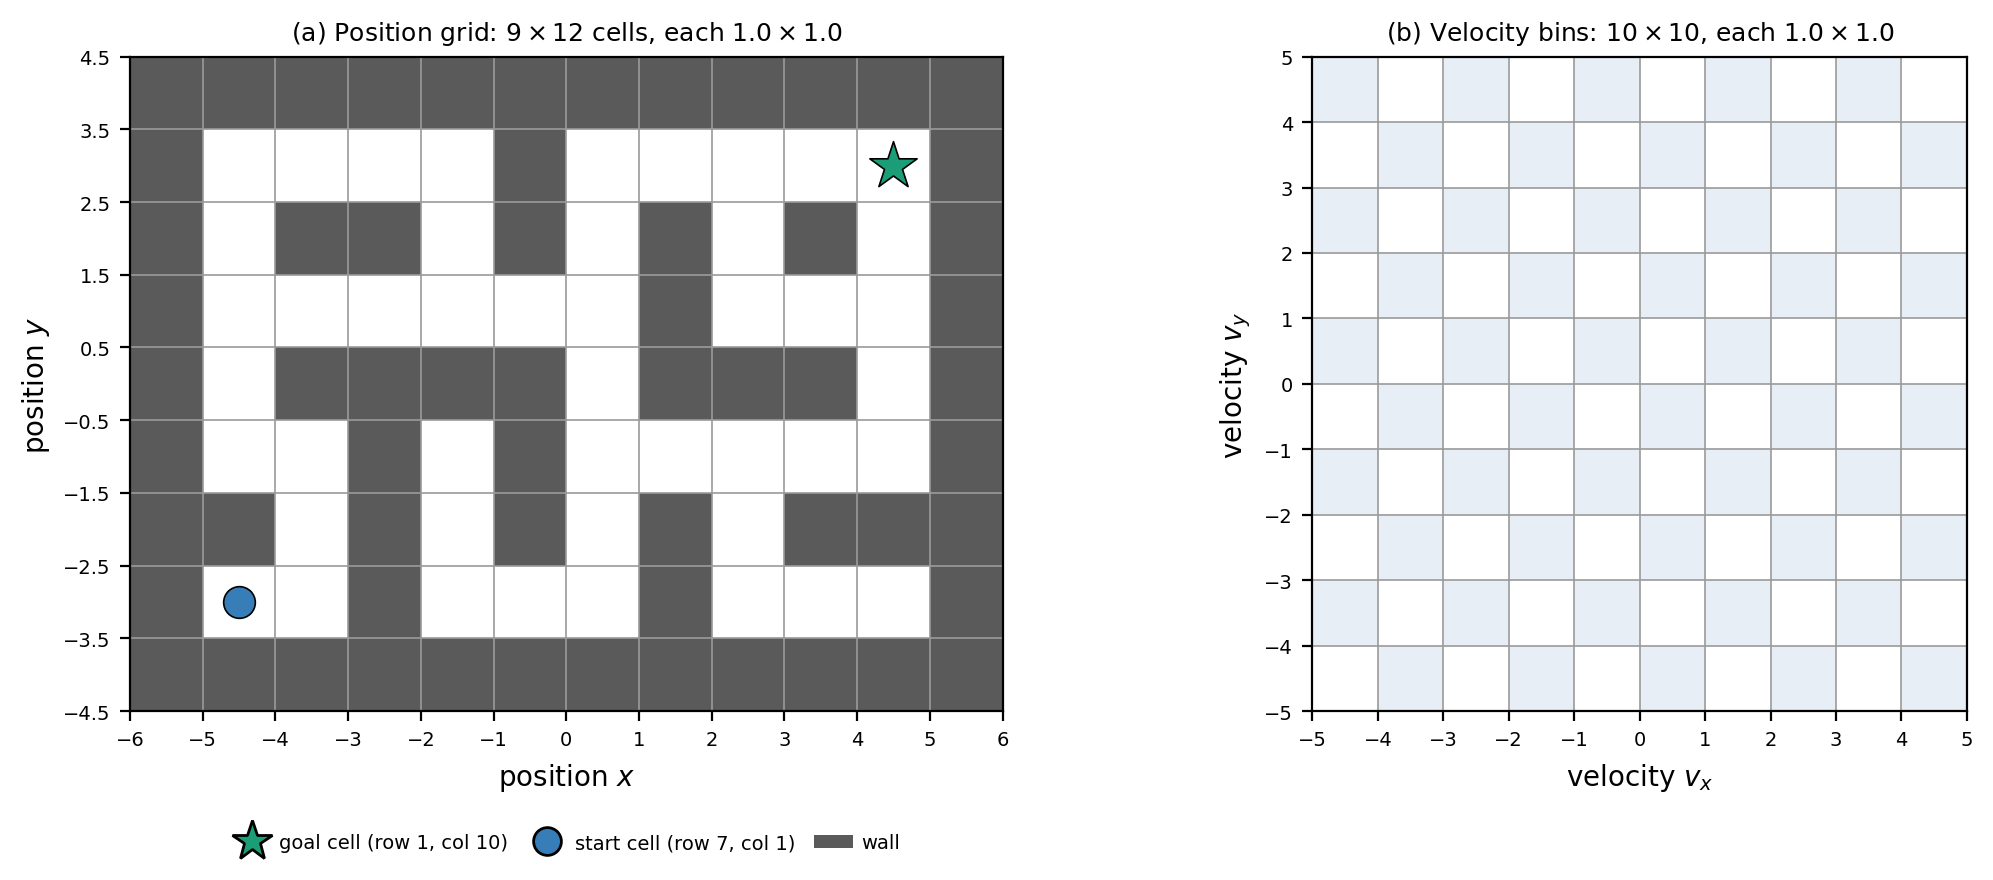
\includegraphics[width=\linewidth]{code/2026-06-23-pointmaze-discretation/pointmaze_discretization.pdf}
\caption{The \texttt{PointMaze\_Large-v3} task and its discretization.
\textbf{(a)} The maze in world coordinates ($x\in[-6,6]$, $y\in[-4.5,4.5]$): gray cells
are walls, white cells are open. The $9\times12$ position grid (cell boundaries drawn at
every $1.0$ unit; each cell is $1.0\times1.0$) is the discretization used by
\texttt{gt\_position}. Visit counts increment only on the $46$ open cells. The sweep sets
\texttt{goal\_position}$=$\texttt{top\_right}, which selects the goal cell (row~1,
col~10) at world $(x,y)=(4.5,3.0)$; the start is the opposite corner, cell (row~7, col~1)
at $(-4.5,-3.0)$. Row~0 is the top of the maze and $y$ increases upward (the same convention as
the visit-count heatmap), so the goal sits at the upper right and the start at the lower left.
\textbf{(b)} The $10\times10$ velocity binning over $(v_x,v_y)\in[-5,5]^2$ (each bin
$1.0\times1.0$, clipped before binning); the faint checkerboard marks bin boundaries.
The joint (position, velocity) cell of \texttt{gt\_position\_velocity}---the ground-truth
field $g$---is the product of (a) and (b), of shape $(9,12,10,10)$.}
\label{fig:pointmaze-discretization}
\end{figure}

\subsection{Fixed start/goal navigation wrappers}
\label{sec:env-nav}

\texttt{FixedStartWrapper}, \texttt{FixedGoalWrapper}, and \texttt{RemoveGoalWrapper} turn the
maze into a deterministic point-to-point task: a fixed start corner, a fixed goal corner,
and the goal removed from the observation.

\begin{table}[H]
\centering
\footnotesize
\begin{tabular}{@{}>{\raggedright\arraybackslash}p{3.4cm} >{\raggedright\arraybackslash}p{3.6cm} >{\raggedright\arraybackslash}p{6.1cm}@{}}
\toprule
\textbf{Hyperparameter} & \textbf{Value} & \textbf{Meaning} \\
\midrule
\texttt{goal\_position} & \texttt{top\_right} (sweep); \texttt{bottom\_left} (script default) & Which corner is the goal: \texttt{bottom\_left} / \texttt{top\_right} / \texttt{random}. \\
\texttt{goal\_cell} & corner cell (row, col) & Goal cell, selected from \texttt{goal\_position}. \\
\texttt{start\_cell} & opposite corner (or seeded) & Fixed start; opposite corner, or seed-chosen when \texttt{random}. \\
\texttt{a\_seed} & $0$--$99$ (sweep) & RNG seed; also picks start/goal when \texttt{random}. \\
\texttt{remove\_keys} & \{desired\_goal, achieved\_goal\} & Observation keys dropped by \texttt{RemoveGoalWrapper}. \\
\bottomrule
\end{tabular}
\caption{Fixed start/goal navigation hyperparameters.}
\label{tab:env-nav}
\end{table}

\subsection{Visit-count instrumentation wrappers}
\label{sec:env-count}

\texttt{PositionVisitCountWrapper} and \texttt{PositionVelocityVisitCountWrapper} track how
often each discretized cell is visited. They supply the counts for the count-based bonuses
and the ground-truth field for the distance metrics.

\begin{table}[H]
\centering
\footnotesize
\begin{tabular}{@{}>{\raggedright\arraybackslash}p{3.4cm} >{\raggedright\arraybackslash}p{3.0cm} >{\raggedright\arraybackslash}p{6.7cm}@{}}
\toprule
\textbf{Hyperparameter} & \textbf{Value} & \textbf{Meaning} \\
\midrule
Position grid & $9\times12$ & Cells for position-only counts. \\
Velocity bins & $10$ per axis & $(v_x,v_y)$ binning over $[-5,5]$. \\
Position count shape & $(9,12)$ & \texttt{gt\_position} count array. \\
Pos+vel count shape & $(9,12,10,10)$ & \texttt{gt\_position\_velocity} count array (the GT). \\
\texttt{update\_counts} & True (train) / False (eval) & Whether stepping increments counts. \\
\texttt{count\_map\_ref} & None (train) / train counts (eval) & Eval reuses the training count array. \\
\bottomrule
\end{tabular}
\caption{Visit-count instrumentation hyperparameters.}
\label{tab:env-count}
\end{table}

\subsection{Intrinsic-reward wrapper}
\label{sec:env-intrinsic}

\texttt{ComputeIntrinsicRewardWrapper} computes the chosen bonus on every step and records it
in \texttt{info}; the bonus is added to the SAC reward inside the replay buffer
(\texttt{VectorIntrinsicReplayBuffer}) as $r = r^{\mathrm{ext}} + \beta\,r^{\mathrm{int}}$.

\begin{table}[H]
\centering
\footnotesize
\begin{tabular}{@{}>{\raggedright\arraybackslash}p{3.4cm} >{\raggedright\arraybackslash}p{3.6cm} >{\raggedright\arraybackslash}p{6.1cm}@{}}
\toprule
\textbf{Hyperparameter} & \textbf{Value} & \textbf{Meaning} \\
\midrule
\texttt{beta} ($\beta$) & $\{10^{-4},\dots,10^{3}\}$ (sweep) & Weight on the intrinsic bonus. \\
\texttt{algorithm} & one of Table~\ref{tab:methods} & Which intrinsic method supplies $r^{\mathrm{int}}$. \\
\texttt{rnd\_obs\_norm} & True & Enable RND input normalization. \\
\texttt{rnd\_distance} & \texttt{mse} & RND per-output distance (\texttt{mse}/\texttt{abs}). \\
\texttt{rnd\_output\_dim} ($m$) & 128 & RND target/predictor output size. \\
\texttt{n\_predictors} ($N$) & 1 & RND ensemble size. \\
\bottomrule
\end{tabular}
\caption{Intrinsic-reward wrapper hyperparameters.}
\label{tab:env-intrinsic}
\end{table}

\subsection{Time-limit termination wrapper}
\label{sec:env-term}

\texttt{TerminateOnTimeLimitWrapper} optionally converts a time-limit truncation into a
termination, so a timeout ends the episode as a full termination rather than a truncation.

\begin{table}[H]
\centering
\footnotesize
\begin{tabular}{@{}>{\raggedright\arraybackslash}p{3.8cm} >{\raggedright\arraybackslash}p{3.0cm} >{\raggedright\arraybackslash}p{6.3cm}@{}}
\toprule
\textbf{Hyperparameter} & \textbf{Value} & \textbf{Meaning} \\
\midrule
\texttt{apply\_termination\_wrapper} & False (sweep / 04); True (script 03) & Treat truncation as termination when on. \\
\bottomrule
\end{tabular}
\caption{Time-limit termination hyperparameters.}
\label{tab:env-term}
\end{table}

\subsection{Training and evaluation configuration}
\label{sec:env-loop}

The SAC training and evaluation loop is shared across environments; its hyperparameters
(sweep values) are below.

\begin{table}[H]
\centering
\footnotesize
\begin{tabular}{@{}>{\raggedright\arraybackslash}p{3.6cm} >{\raggedright\arraybackslash}p{2.8cm} >{\raggedright\arraybackslash}p{6.7cm}@{}}
\toprule
\textbf{Hyperparameter} & \textbf{Value} & \textbf{Meaning} \\
\midrule
\texttt{total\_timesteps} & $2{\times}10^{6}$ & Training environment steps per run. \\
\texttt{discount\_factor} ($\gamma$) & 0.999 & SAC discount. \\
\texttt{eval\_freq} & 50000 & Evaluate every this many steps. \\
\texttt{n\_eval\_episodes} & 100 & Episodes per mid-training evaluation. \\
\texttt{n\_eval\_episodes\_final} & 10000 & Episodes at the final evaluation. \\
\texttt{device} & cpu (sweep) & Compute device. \\
Policy & SAC (\texttt{MlpPolicy}) & Stable-Baselines3 agent. \\
\bottomrule
\end{tabular}
\caption{Training and evaluation loop hyperparameters.}
\label{tab:env-loop}
\end{table}

%==============================================================================
\section{Optimizer for the RND predictor}
\label{sec:optimizer}
%==============================================================================

The RND bonus at a state is the predictor's residual error there
(Section~\ref{sec:rnd}), so how fast that error shrinks as a state is revisited
is set entirely by the optimizer that fits the predictor $g_\phi$ to the frozen
target $f_\theta$. Section~\ref{sec:opt-defs} builds the optimizers up from their
definitions and asks which of them makes the learned bonus fall off like the
count oracle's $1/\sqrt{n}$; Section~\ref{sec:opt-used} then records the optimizer
this project and the widely-used RND code actually use.

\subsection{Optimizers from first principles}
\label{sec:opt-defs}

\paragraph{Why optimizers matter for exploration bonuses.}
For ordinary RND, the intrinsic bonus is the prediction error between a trainable
predictor $g_\phi$ and a frozen random target $f_\theta$:
\[
e_\phi(\tilde{x})
=
g_\phi(\tilde{x})-f_\theta(\tilde{x}).
\]
The target network $f_\theta$ never changes. Only the predictor parameters
$\phi$ are trained. Therefore, the speed at which the bonus decreases at a
visited input is controlled by the optimizer used to update $\phi$.

If the optimizer makes the predictor forget old visits, then the RND bonus will
not behave like a count. If the optimizer accumulates information from all visits,
then the RND bonus can become closer to the count oracle's $1/\sqrt{n}$ decay.

\begin{definition}[Optimizer]
An optimizer is an update rule for the trainable parameters $\phi$. At update
step $t$, the optimizer receives a minibatch loss $L_t(\phi)$ and its gradient
\[
h_t=\nabla_\phi L_t(\phi_t).
\]
The optimizer then produces the next parameters $\phi_{t+1}$. In the simplest
case, the update has the form
\[
\phi_{t+1}=\phi_t-\eta h_t,
\]
where $\eta>0$ is the learning rate.
\end{definition}

\paragraph{The RND predictor loss.}
For a minibatch of $b$ RND inputs $\{x_i\}_{i=1}^{b}$, where $x_i$ may be
$s_i$, $s_i'$, $[s_i;a_i]$, or $[s_i;a_i;s_i']$ depending on the RND variant, the
predictor is trained to minimize
\begin{align}
L_t(\phi)
=
\frac1b\sum_{i=1}^{b}
\frac12
\left\lVert
g_\phi(\tilde{x}_i)-f_\theta(\tilde{x}_i)
\right\rVert_2^2.
\end{align}
The gradient $h_t=\nabla_\phi L_t(\phi_t)$ tells us how to change $\phi$ to make
the predictor closer to the frozen target on the current minibatch.

\paragraph{Gradient descent and stochastic gradient descent.}
The most basic optimizer is gradient descent:
\begin{align}
\phi_{t+1}
=
\phi_t-\eta h_t.
\end{align}
The gradient points in the direction of steepest increase of the loss, so the
optimizer subtracts the gradient to move downhill. In deep learning we usually use
a minibatch instead of the whole dataset; this is called stochastic gradient
descent, or SGD. The update formula is the same, but $h_t$ is a noisy minibatch
gradient.

For RND, constant-learning-rate SGD has one important weakness: it does not keep a
true count of how many times a state has been visited. It keeps moving with the
same step size $\eta$, so under minibatch noise the predictor error typically
falls quickly at first and then reaches a nonzero steady-state error.

\paragraph{Momentum.}
Momentum smooths the gradient by keeping a velocity-like variable:
\begin{align}
v_t &= \rho v_{t-1}+h_t,\\
\phi_{t+1} &= \phi_t-\eta v_t,
\qquad 0\le\rho<1.
\end{align}
Momentum is useful when consecutive gradients point in similar directions: it
accelerates motion in stable directions and damps small oscillations. However, if
$\eta$ is constant, momentum is still a constant-gain method. It improves
optimization speed, but it does not by itself create a count-like $1/\sqrt{n}$
bonus.

\paragraph{RMSProp.}
RMSProp rescales each parameter by a moving average of squared gradients:
\begin{align}
q_t
&=
\rho q_{t-1}+(1-\rho)(h_t\odot h_t),\\
\phi_{t+1}
&=
\phi_t
-
\eta\,
\frac{h_t}{\sqrt{q_t}+\epsilon}.
\end{align}
Here $\odot$ means element-wise multiplication, and the division is also
element-wise. RMSProp gives smaller steps to parameters with consistently large
gradients and larger steps to parameters with consistently small gradients. The
important word is ``moving'': $q_t$ is an exponential moving average, so old
gradients are gradually forgotten. Thus RMSProp is adaptive, but it is not a
lifetime-count optimizer.

\paragraph{Adam.}
Adam combines momentum and RMSProp. To avoid confusion with the intrinsic reward
coefficient $\beta$, write Adam's two decay rates as $\rho_1$ and $\rho_2$:
\begin{align}
m_t
&=
\rho_1 m_{t-1}+(1-\rho_1)h_t,\\
q_t
&=
\rho_2 q_{t-1}+(1-\rho_2)(h_t\odot h_t),\\
\widehat{m}_t
&=
\frac{m_t}{1-\rho_1^t},
\qquad
\widehat{q}_t
=
\frac{q_t}{1-\rho_2^t},\\
\phi_{t+1}
&=
\phi_t
-
\eta
\frac{\widehat{m}_t}{\sqrt{\widehat{q}_t}+\epsilon}.
\end{align}
Adam is the standard default optimizer for many neural networks because it is
stable and fast. The current RND predictor uses constant-rate Adam with its own
learning rate. But Adam also uses exponential moving averages. Therefore, Adam
does not remember the total number of visits to an input. This means it can make
the RND bonus saturate instead of continuing to decay like $1/\sqrt{n}$.

\paragraph{AdaGrad.}
AdaGrad is different because it uses a cumulative sum of squared gradients:
\begin{align}
c_t
&=
c_{t-1}+h_t\odot h_t,\\
\phi_{t+1}
&=
\phi_t
-
\eta
\frac{h_t}{\sqrt{c_t}+\epsilon}.
\end{align}
Unlike Adam and RMSProp, the accumulator $c_t$ does not forget old gradients. If
the same input, or the same feature direction, appears many times, then the
corresponding entries of $c_t$ grow. The effective step size shrinks roughly like
\[
\frac{1}{\sqrt{c_t}}.
\]
This makes AdaGrad the closest off-the-shelf optimizer to a soft count. It is not
an exact per-state counter, because neural-network parameters are shared across
states, but it is much closer to count accumulation than Adam.

\paragraph{A $1/t$ learning-rate schedule.}
Another way to obtain count-like behavior is to use a decreasing learning rate:
\begin{align}
\eta_t
=
\frac{\eta_0}{t+t_0},
\qquad
\phi_{t+1}
=
\phi_t-\eta_t h_t.
\end{align}
This is the classical stochastic-approximation idea: early updates move a lot,
while later updates average more and more slowly. In the idealized case where the
same state is visited $n$ times and the predictor behaves like a local average,
a $1/n$ step size gives an error norm that decays like
\[
\lVert e_n\rVert_2\propto \frac1{\sqrt{n}}.
\]
This matches the count oracle's bonus scale.

\paragraph{Polyak--Ruppert averaging.}
Polyak--Ruppert averaging keeps training with noisy updates, but uses the average
of the iterates for prediction:
\begin{align}
\bar{\phi}_t
=
\frac1t\sum_{k=1}^{t}\phi_k.
\end{align}
The predictor readout becomes $g_{\bar{\phi}_t}$ rather than $g_{\phi_t}$. The
averaging can reduce the variance of the final predictor. In simple stochastic
approximation problems, the averaged iterate has the desired
$1/\sqrt{n}$ statistical error rate. This makes it a useful optimizer variant to
test for RND, especially for the linear RND head.

\paragraph{Why constant Adam does not give a count bonus.}
Consider one fixed input $x$ that has been included in $n$ predictor updates.
Let
\[
e_n=g_\phi(\tilde{x})-f_\theta(\tilde{x})
\]
be the RND residual at that input after its $n$-th relevant update. A local
linear approximation gives the recursion
\begin{align}
e_{n+1}
\approx
(I-\eta_n K)e_n+\eta_n\xi_n,
\end{align}
where $K$ is the local tangent-kernel curvature and $\xi_n$ represents noise from
other samples in the minibatch.

With a constant effective step size $\eta_n=\eta$, the deterministic part can
decrease quickly, but the noise term keeps injecting error. The residual typically
approaches a nonzero steady-state level:
\[
\mathbb{E}\lVert e_n\rVert_2^2
\longrightarrow
\text{constant depending on }\eta.
\]
So the bonus stops decreasing.

With a count-like step size $\eta_n\propto 1/n$, the recursion behaves like a
running average:
\[
\mathbb{E}\lVert e_n\rVert_2^2
=
O\!\left(\frac1n\right),
\qquad
\lVert e_n\rVert_2
=
O\!\left(\frac1{\sqrt{n}}\right).
\]
Thus the \emph{L2 residual} has the same scaling as the count oracle. If the
bonus is instead the squared loss
\[
d(x)=\frac12\lVert e_n\rVert_2^2,
\]
then the bonus decays like $1/n$, not $1/\sqrt{n}$. Therefore, optimizer choice
and bonus readout must be tested together.

\paragraph{Important distinction: error norm versus squared error.}
The count oracle uses
\[
r^{\mathrm{int}}(n)=\min(1,n^{-1/2}),
\]
which is a standard-deviation-scale quantity. Therefore, the matching learned
quantity is the residual norm
\[
\lVert g_\phi(\tilde{x})-f_\theta(\tilde{x})\rVert_2.
\]
The default RND squared-error bonus
\[
\frac12\lVert g_\phi(\tilde{x})-f_\theta(\tilde{x})\rVert_2^2
\]
is variance-scale. If the norm decays as $1/\sqrt{n}$, the squared error decays
as $1/n$. This is why the next optimizer experiments should include both the
optimizer and the readout type.

\begin{table}[H]
\centering
\footnotesize
\setlength{\tabcolsep}{3.5pt}
\renewcommand{\arraystretch}{1.35}
\begin{tabular}{@{}>{\raggedright\arraybackslash}p{2.6cm} >{\raggedright\arraybackslash}p{4.1cm} >{\raggedright\arraybackslash}p{3.2cm} >{\centering\arraybackslash}p{1.2cm}@{}}
\toprule
\textbf{Optimizer} & \textbf{Memory used by the update} & \textbf{Expected RND-bonus behavior} & \textbf{Count-like?} \\
\midrule
SGD, constant $\eta$ &
No memory except current $\phi_t$ &
Fast early decrease, then possible steady-state residual &
\xmark \\
\midrule
Momentum &
Exponential moving average of gradients &
Smoother and faster than SGD, but still constant-gain &
\xmark \\
\midrule
RMSProp &
Exponential moving average of squared gradients &
Adaptive scale, but old visits are forgotten &
\xmark \\
\midrule
Adam &
Exponential moving average of gradients and squared gradients &
Stable default; likely bonus saturation with constant $\eta$ &
\xmark \\
\midrule
AdaGrad &
Cumulative sum of squared gradients &
Soft feature-count behavior; step shrinks with repeated visits &
$\approx$ \\
\midrule
SGD with $\eta_t=\eta_0/(t+t_0)$ &
Global decreasing step size &
Can produce $1/\sqrt{n}$ residual decay in the ideal local-average case &
\cmark \\
\midrule
Polyak--Ruppert averaging &
Average of past iterates &
Can recover $1/\sqrt{n}$ statistical error while using noisy updates &
\cmark \\
\bottomrule
\end{tabular}
\caption{Optimizer families for the RND predictor. The main issue for exploration
is not only whether the loss goes down, but whether the residual behaves like a
count-based uncertainty estimate.}
\label{tab:optimizer-from-definition}
\end{table}

\paragraph{Optimizer conclusion.}
Adam is a good default for making neural-network losses decrease, but it is not
designed to represent visit counts. For RND as an exploration bonus, the next
experiments should test count-aware alternatives: AdaGrad, SGD with a $1/t$
schedule, and Polyak--Ruppert averaging. These should be paired with an L2
residual readout when the goal is to match the count oracle's $1/\sqrt{n}$ scale.

\subsection{Optimizers used in practice}
\label{sec:opt-used}

Every RND implementation we examined trains the predictor with Adam
\citep{kingma2014adam}; Table~\ref{tab:opt-used} lists the settings. They agree
on betas $(0.9,0.999)$ and zero weight decay and differ only in the columns
shown. The original RND line of work---the paper \citep{burda2019exploration},
OpenAI's release, the most-used PyTorch port, and CleanRL---folds the predictor
into the \emph{same} Adam as the PPO policy at learning rate $10^{-4}$. This
project and RLeXplore instead give the predictor its \emph{own} Adam at
$10^{-3}$, because SAC \citep{haarnoja2018soft} is off-policy and the predictor
is fit on replay minibatches rather than on-policy rollouts. The fact that
matters for Section~\ref{sec:opt-defs}: none of them anneal the predictor's
learning rate on a $1/n$ schedule and none use a cumulative (AdaGrad-style)
step---the learning rate is constant throughout (CleanRL's optional
linear-to-zero anneal is the only schedule, and it decays faster than $1/n$, not
slower).

\begin{table}[H]
\centering
\footnotesize
\setlength{\tabcolsep}{3.5pt}
\renewcommand{\arraystretch}{1.2}
\begin{tabular}{@{}>{\raggedright\arraybackslash}p{3.0cm} >{\raggedright\arraybackslash}p{0.9cm} >{\raggedright\arraybackslash}p{1.7cm} >{\raggedright\arraybackslash}p{3.4cm} >{\raggedright\arraybackslash}p{1.5cm} >{\raggedright\arraybackslash}p{1.6cm}@{}}
\toprule
\textbf{Source} & \textbf{Optim.} & \textbf{LR / $\epsilon$} & \textbf{Optimizer scope} & \textbf{Grad.\ clip} & \textbf{LR schedule} \\
\midrule
This work (\sout{\texttt{04\_many\_\allowbreak exploration\_\allowbreak method}}\claudeedit{\texttt{train.py}}) & Adam & $10^{-3}$ / $10^{-8}$ & own (predictor only) & none & none \\
RLeXplore \texttt{rllte} (\sout{\texttt{02\_rnd\_\allowbreak rlexplore}}\claudeedit{\texttt{legacy/02\_rnd\_\allowbreak rlexplore}}) & Adam & $10^{-3}$ / $10^{-8}$ & own (predictor only) & none & none \\
\multicolumn{6}{@{}>{\raggedright\arraybackslash}p{12cm}@{}}{\claudecomment{driver renamed to train.py and the 02 precursor archived under legacy/ in the reorganization}} \\
\midrule
Burda et al.\ 2019 (paper) & Adam & $10^{-4}$ / n/s & shared with PPO & n/s & none \\
OpenAI repo & Adam (MPI) & $10^{-4}$ / $10^{-8}$ & shared (policy\,+\,value\,+\,predictor) & global-norm $1.0$ & none \\
jcwleo (PyTorch) & Adam & $10^{-4}$ / $10^{-8}$ & shared with PPO & global-norm $0.5$ & none \\
CleanRL \texttt{ppo\_rnd\_\allowbreak envpool} & Adam & $10^{-4}$ / $10^{-5}$ & shared with PPO & global-norm $0.5$ & linear $\to 0$ \\
\bottomrule
\end{tabular}
\caption{Optimizer used to train the RND predictor network. All sources use Adam
\citep{kingma2014adam} with betas $(0.9,0.999)$ and no weight decay; the columns
list only what differs (``$\epsilon$'' is the Adam epsilon). ``Optimizer scope''
is whether the predictor has its own Adam or shares one optimizer with the PPO
policy and value networks (so the predictor's learning rate equals the policy's).
n/s = not stated in the paper. The top block is this project's stack; the bottom
block is the original RND paper and the three most-used RND repositories.}
\label{tab:opt-used}
\end{table}

\noindent{\footnotesize Source files:
RLeXplore \url{https://github.com/RLE-Foundation/rllte} (\texttt{rllte/xplore/reward/rnd.py});
OpenAI \url{https://github.com/openai/random-network-distillation} (\texttt{ppo\_agent.py}, \texttt{run\_atari.py});
jcwleo \url{https://github.com/jcwleo/random-network-distillation-pytorch} (\texttt{agents.py}, \texttt{config.conf});
CleanRL \url{https://github.com/vwxyzjn/cleanrl} (\texttt{ppo\_rnd\_envpool.py}, also vendored here as \texttt{07\_reconstruction/ppo\_rnd\_envpool.py}).}

%==============================================================================
\section{Logging}
\label{sec:logging}
%==============================================================================

Every training run records its metrics to \textbf{its own JSON file} under
\texttt{train\_\allowbreak runs/<run>/\allowbreak data/local/}. Because each run owns a distinct file, the
$512$ concurrent work-queue workers never write the same path, so there is \textbf{no file-lock
contention}. File access is slow, so logging is \textbf{group-style and written once}: every metric is
accumulated in memory by its callback at the evaluation cadence (\texttt{eval\_freq}) during training, and
the whole record --- all groups --- is flushed in a \textbf{single file write at the end of the run}. No
metric is written incrementally per step.

\paragraph{Run id (filename convention).}
The local work queue replaces the W\&B sweep as the config source. Each run carries an integer
\texttt{run\_id} $\in\{0,\dots,\texttt{run\_total}-1\}$ giving its position in the sweep, and
\texttt{run\_total} (here $600$); together \texttt{run\_id}/\texttt{run\_total} is the run's identity and
names its JSON file (e.g.\ \texttt{042\_of\_600.json}). The sweep iterates the \textbf{seed outermost}:
seed $s$ owns a contiguous id block of one id per algorithm in fixed order (\texttt{gt\_\allowbreak
position\_\allowbreak velocity}, \texttt{rnd\_\allowbreak elliptical}, \texttt{rnd\_\allowbreak state}), so
seed $0$ takes ids $0$--$2$, seed $1$ takes $3$--$5$, and an earlier seed always has smaller ids than a
later one.

\paragraph{What is logged.}
Table~\ref{tab:logging} lists every logged quantity by group. A \emph{group} is the set of metrics written
together as one JSON list; grouping is what minimizes the number of slow file writes. An
\emph{intermediate} metric is captured at every \texttt{eval\_freq} step (one snapshot appended to its
group's list) and persisted at the final write; a \emph{final} field is written once at run end.

\begin{table}[H]
\centering
\footnotesize
\setlength{\tabcolsep}{3pt}
\renewcommand{\arraystretch}{1.3}
\begin{tabular}{@{}>{\raggedright\arraybackslash}p{2.5cm} >{\raggedright\arraybackslash}p{1.8cm} >{\raggedright\arraybackslash}p{2.0cm} >{\raggedright\arraybackslash}p{1.4cm} >{\raggedright\arraybackslash}p{2.3cm} >{\raggedright\arraybackslash}p{2.2cm}@{}}
\toprule
\textbf{Quantity} & \textbf{Parameters} & \textbf{Position (cadence)} & \textbf{Group} & \textbf{Purpose} & \textbf{Trigger (when / when not)} \\
\midrule
\texttt{run\_\allowbreak id}, \texttt{run\_\allowbreak total} & sweep position \& size & final (once at run end) & top-level & the run's identity $i/\text{total}$; names its JSON file & every run \\
\addlinespace
\texttt{algorithm}, \texttt{beta}, \texttt{a\_\allowbreak seed}, \texttt{z\_\allowbreak logging\_\allowbreak mode}, \texttt{total\_\allowbreak timesteps}, \texttt{eval\_\allowbreak freq}, \texttt{runtime\_\allowbreak seconds} & the run's argparse config + dispatch mode + wall clock & final (once at run end) & top-level & identify, reproduce, and group runs; per-run timing & every run \\
\midrule
\texttt{eval/\allowbreak mean\_\allowbreak extrinsic\_\allowbreak reward} ($+$ intrinsic, total, \texttt{ep\_\allowbreak length}); \texttt{eval/\allowbreak n\_\allowbreak eval\_\allowbreak episodes} & a fresh eval rollout of \texttt{n\_\allowbreak eval\_\allowbreak episodes} ($=100$; \texttt{\ldots\_final} at the last step) & intermediate, every \texttt{eval\_\allowbreak freq} ($50$k steps) $+$ a final eval at \texttt{total\_\allowbreak timesteps} & \texttt{eval\_\allowbreak history} & primary metric (final extrinsic reward) and the eval reward curve & every algorithm, every eval step \\
\addlinespace
\texttt{visit\_\allowbreak counts/}\{\texttt{total\_\allowbreak visits}, \texttt{cells\_\allowbreak visited}, \texttt{open\_\allowbreak cells}, \texttt{coverage\_\allowbreak pct}\} & the visit-count env over the eval rollout & intermediate, every \texttt{eval\_\allowbreak freq} & \texttt{eval\_\allowbreak history} & maze coverage / exploration breadth & only when a visit-count env is attached (all run-2 algos) \\
\midrule
\texttt{train/\allowbreak mean\_\allowbreak extrinsic\_\allowbreak reward} ($+$ intrinsic, total, \texttt{episode\_\allowbreak length}); \texttt{train/\allowbreak n\_\allowbreak episodes\_\allowbreak averaged} & the past \texttt{n\_\allowbreak eval\_\allowbreak episodes} ($=100$) completed training episodes & intermediate, every \texttt{eval\_\allowbreak freq} & \texttt{train\_\allowbreak history} & training-time performance (the dashed training curve) & every algorithm, every eval step \\
\midrule
\texttt{distance\_\allowbreak to\_\allowbreak gt/}\{\texttt{min\_\allowbreak c\_\allowbreak l1\_\allowbreak diff}, \texttt{min\_\allowbreak c\_\allowbreak l2\_\allowbreak diff}, \texttt{min\_\allowbreak c\_\allowbreak l1\_\allowbreak inv}, \texttt{min\_\allowbreak c\_\allowbreak l2\_\allowbreak inv}, \texttt{normalized\_\allowbreak l2}, \texttt{normalized\_\allowbreak angle\_\allowbreak rad}\} & the learned bonus field vs the oracle \texttt{gt\_\allowbreak position\_\allowbreak velocity} visit-count field & intermediate, every \texttt{eval\_\allowbreak freq} & \texttt{distance\_\allowbreak history} & how close the learned bonus field is to the oracle (the core research metric) & \textbf{only} algorithms in \texttt{ALGORITHMS\_\allowbreak NO\_\allowbreak ACTION} (e.g.\ \texttt{gt\_\allowbreak position\_\allowbreak velocity}, \texttt{rnd\_\allowbreak state}); \textbf{not} \texttt{rnd\_\allowbreak elliptical} \\
\bottomrule
\end{tabular}
\caption{What each run logs to its own per-run JSON, by group. All metrics are accumulated in memory at
the evaluation cadence and written in a single file access at the end of the run (group-style logging, to
minimize slow file access); one file per run avoids lock contention across the $512$ concurrent workers.
\emph{Intermediate} $=$ one snapshot per \texttt{eval\_freq} step appended to the group's list;
\emph{final} $=$ written once at run end. The \texttt{distance\_history} group is the only one with an
algorithm-dependent trigger: it is logged only for algorithms whose intrinsic bonus is a state-only field
(\texttt{ALGORITHMS\_NO\_ACTION}), which excludes \texttt{rnd\_elliptical}.}
\label{tab:logging}
\end{table}

%==============================================================================
% Train-run-1 content assembled from the analysis folder
%   ../train_runs/2026-06-24-17-31_run_1_before_reorganization/analysis/
% Data table tab:trainrun1-best is spliced by code/03_table_and_bar.py (markers below);
% figures bar_*/line_* are produced by code/03_table_and_bar.py and code/04_line_plot.py.
%==============================================================================
\section{Train runs}
\label{sec:train-runs}
%==============================================================================

This section reports the SAC training runs that sweep the intrinsic-bonus methods
of Section~\ref{sec:methods} on \texttt{PointMaze\_Large-v3}, and ranks the methods
by the extrinsic reward they reach.

\subsection{Train run 1 (before reorganization)}
\label{sec:train-run-1}

\paragraph{Sweep.}
Train run~1 is the Weights \& Biases grid sweep \texttt{sweep\_my\_rnd}
(id \texttt{y24vyh06}, project \texttt{rnd\_07\_reconstruction}). It crosses every
intrinsic-bonus method of Table~\ref{tab:methods} with eight intrinsic
coefficients~$\beta$ and up to 100 random seeds, all on the same environment and
SAC configuration of Section~\ref{sec:environments}---with the fixed
\texttt{bottom\_right} goal used here, before the later reorganization to
\texttt{top\_right}. The fixed (non-swept) hyperparameters are listed in
Table~\ref{tab:trainrun1-fixed} and the swept axes in
Table~\ref{tab:trainrun1-sweep}; the fixed values are the sweep configuration of
Section~\ref{sec:environments} (notably $2\times10^{6}$ training steps, discount
$\gamma=0.999$, and a final evaluation over $10^{4}$ episodes). Of the $8000$
launched runs, $3292$ finished and $4708$ crashed; only finished runs enter the
aggregates below.

% Fixed (non-swept) hyperparameters of train run 1 — values verified from the
% data/y24vyh06 run configs (hand-authored static config).
\begin{table}[H]
\centering
\footnotesize
\setlength{\tabcolsep}{5pt}
\renewcommand{\arraystretch}{1.2}
\begin{tabular}{@{}>{\raggedright\arraybackslash}p{4.0cm} >{\raggedright\arraybackslash}p{4.6cm} >{\raggedright\arraybackslash}p{3.9cm}@{}}
\toprule
\textbf{Hyperparameter} & \textbf{Symbol} & \textbf{Value} \\
\midrule
Environment & \texttt{env\_name} & \texttt{PointMaze\_Large-v3} \\
Goal corner & \texttt{goal\_position} & \texttt{bottom\_right} \\
Continuing task & \texttt{continuing\_task} & True \\
Reset target on goal & \texttt{reset\_target} & False \\
Max episode steps & \texttt{env\_max\_episode} & $400$ \\
Time-limit $\to$ termination & \texttt{apply\_\allowbreak termination\_\allowbreak wrapper} & False \\
\midrule
Training steps & \texttt{total\_timesteps} & $2\times10^{6}$ \\
Discount factor & $\gamma$ & $0.999$ \\
Policy / agent & --- & SAC (\texttt{MlpPolicy}) \\
Compute device & \texttt{device} & \texttt{cpu} \\
Evaluation frequency & \texttt{eval\_freq} & every $50000$ steps \\
Eval episodes (mid-training) & \texttt{n\_eval\_episodes} & $100$ \\
Eval episodes (final) & \texttt{n\_eval\_\allowbreak episodes\_\allowbreak final} & $10^{4}$ \\
\midrule
RND input normalization & \texttt{rnd\_obs\_norm} & True \\
RND distance & \texttt{rnd\_distance} & \texttt{mse} \\
RND output dimension & $m$ & $128$ \\
RND ensemble size & $N$ & $1$ \\
\bottomrule
\end{tabular}
\caption{Fixed (non-swept) hyperparameters of train run~1 (\texttt{y24vyh06}), held
constant across the grid of Table~\ref{tab:trainrun1-sweep}. Values are read from the
run configurations and match the sweep settings of Section~\ref{sec:environments}; the
goal is \texttt{bottom\_right} here, before the later reorganization to
\texttt{top\_right}.}
\label{tab:trainrun1-fixed}
\end{table}

\begin{table}[H]
\centering
\footnotesize
\setlength{\tabcolsep}{5pt}
\renewcommand{\arraystretch}{1.2}
\begin{tabular}{@{}>{\raggedright\arraybackslash}p{3.4cm} >{\raggedright\arraybackslash}p{2.1cm} >{\raggedright\arraybackslash}p{7.0cm}@{}}
\toprule
\textbf{Hyperparameter} & \textbf{Symbol} & \textbf{Swept values} \\
\midrule
Intrinsic-bonus method & \texttt{algorithm} & The $10$ methods of Table~\ref{tab:methods}: \texttt{no\_exploration}; \texttt{gt\_position}, \texttt{gt\_position\_velocity}; \texttt{rnd\_next\_state}, \texttt{rnd\_next\_state\_position\_only}, \texttt{rnd\_state}, \texttt{rnd\_state\_action}, \texttt{rnd\_state\_action\_next\_state}, \texttt{rnd\_linear\_next\_state}; \texttt{rnd\_elliptical}. \\
Intrinsic coefficient & $\beta$ & $\{10^{-4},\,10^{-3},\,10^{-2},\,10^{-1},\,1,\,10,\,10^{2},\,10^{3}\}$ ($8$ values; forced to $0$ for \texttt{no\_exploration}). \\
Random seed & \texttt{a\_seed} & $0$--$99$; seeds \texttt{random}, \texttt{numpy}, \texttt{torch}, CUDA together ($\approx 40$ finished seeds per (\texttt{algorithm}, $\beta$) group). \\
\bottomrule
\end{tabular}
\caption{Swept axes of train run~1 (\texttt{y24vyh06}). The grid is
\texttt{algorithm} $\times\,\beta\,\times$ \texttt{a\_seed}; all other knobs are the
Section~\ref{sec:environments} sweep values.}
\label{tab:trainrun1-sweep}
\end{table}

\paragraph{Aggregation.}
Finished runs are grouped by $(\texttt{algorithm}, \beta)$. The primary metric is
the final eval extrinsic reward $r^{\mathrm{ext}}$ (the $10^{4}$-episode evaluation
at $2\times10^{6}$ steps). For a group of $n$ seeds with per-seed final rewards
$R_i$, we report the seed mean and its standard error,
\begin{align}
\bar{R} = \frac{1}{n}\sum_{i=1}^{n} R_i,
\qquad
\mathrm{SE} = \frac{s}{\sqrt{n}},
\qquad
s = \sqrt{\frac{1}{n-1}\sum_{i=1}^{n}\big(R_i-\bar{R}\big)^2}.
\end{align}
For each algorithm we keep the single coefficient
$\beta^\star = \argmax_{\beta}\,\bar{R}(\texttt{algorithm},\beta)$ with the largest
mean reward---the best-tuned coefficient---and report that group.
Table~\ref{tab:trainrun1-best} lists $\beta^\star$ and its $(\bar{R},\mathrm{SE},n)$
per algorithm.

\begin{table}[H]
\centering
\footnotesize
\setlength{\tabcolsep}{8pt}
\renewcommand{\arraystretch}{1.2}
% Auto-generated by ../train_runs/2026-06-24-17-31_run_1_before_reorganization/analysis/code/03_table_and_bar.py
% >>> AUTO-GENERATED TABLE START: trainrun1-best
\begin{tabular}{@{}>{\raggedright\arraybackslash}p{5.2cm} r r r r@{}}
\toprule
\textbf{Algorithm} & \textbf{$\beta^\star$} & \textbf{$\bar{R}$ ($\downarrow$)} & \textbf{SE} & \textbf{$n$} \\
\midrule
\texttt{gt\_position\_velocity} & $1$ & \textbf{74.86} & 4.63 & 43 \\
\texttt{rnd\_elliptical} & $0.01$ & \underline{71.12} & 6.09 & 44 \\
\texttt{rnd\_state} & $100$ & 69.90 & 4.80 & 41 \\
\texttt{rnd\_next\_state} & $100$ & 62.03 & 5.34 & 40 \\
\texttt{gt\_position} & $10$ & 59.37 & 5.32 & 45 \\
\texttt{rnd\_state\_action\_next\_state} & $100$ & 57.04 & 4.97 & 40 \\
\texttt{rnd\_state\_action} & $10$ & 52.53 & 4.87 & 43 \\
\texttt{rnd\_linear\_next\_state} & $10$ & 32.18 & 5.60 & 42 \\
\texttt{rnd\_next\_state\_position\_only} & $1000$ & 29.99 & 5.97 & 38 \\
\texttt{no\_exploration} & $0.0001$ & 25.60 & 6.09 & 45 \\
\bottomrule
\end{tabular}
% <<< AUTO-GENERATED TABLE END: trainrun1-best
\caption{Train run~1: best intrinsic coefficient $\beta^\star$ per algorithm, with
the final eval extrinsic reward $\bar{R}$ (mean over $n$ finished seeds),
its standard error, and $n$. Rows are sorted by $\bar{R}$ descending;
the best value is \textbf{bold} and the second best is \underline{underlined}.
Higher reward is better.}
\label{tab:trainrun1-best}
\end{table}

\paragraph{Final performance.}
Figure~\ref{fig:trainrun1-bar} ranks the algorithms by the best-$\beta^\star$ mean
eval reward $\bar{R}$ with standard-error bars. The
\texttt{gt\_position\_velocity} count oracle is the strongest method
($\bar{R}=74.9$), with the learned \texttt{rnd\_elliptical} bonus a close second
($71.1$) and \texttt{rnd\_state} third ($69.9$); all three are well above the
\texttt{no\_exploration} baseline ($25.6$). The position-only RND variants and the
linear RND head trail the field.

\begin{figure}[H]
\centering
% Plot produced by ../train_runs/2026-06-24-17-31_run_1_before_reorganization/analysis/code/03_table_and_bar.py
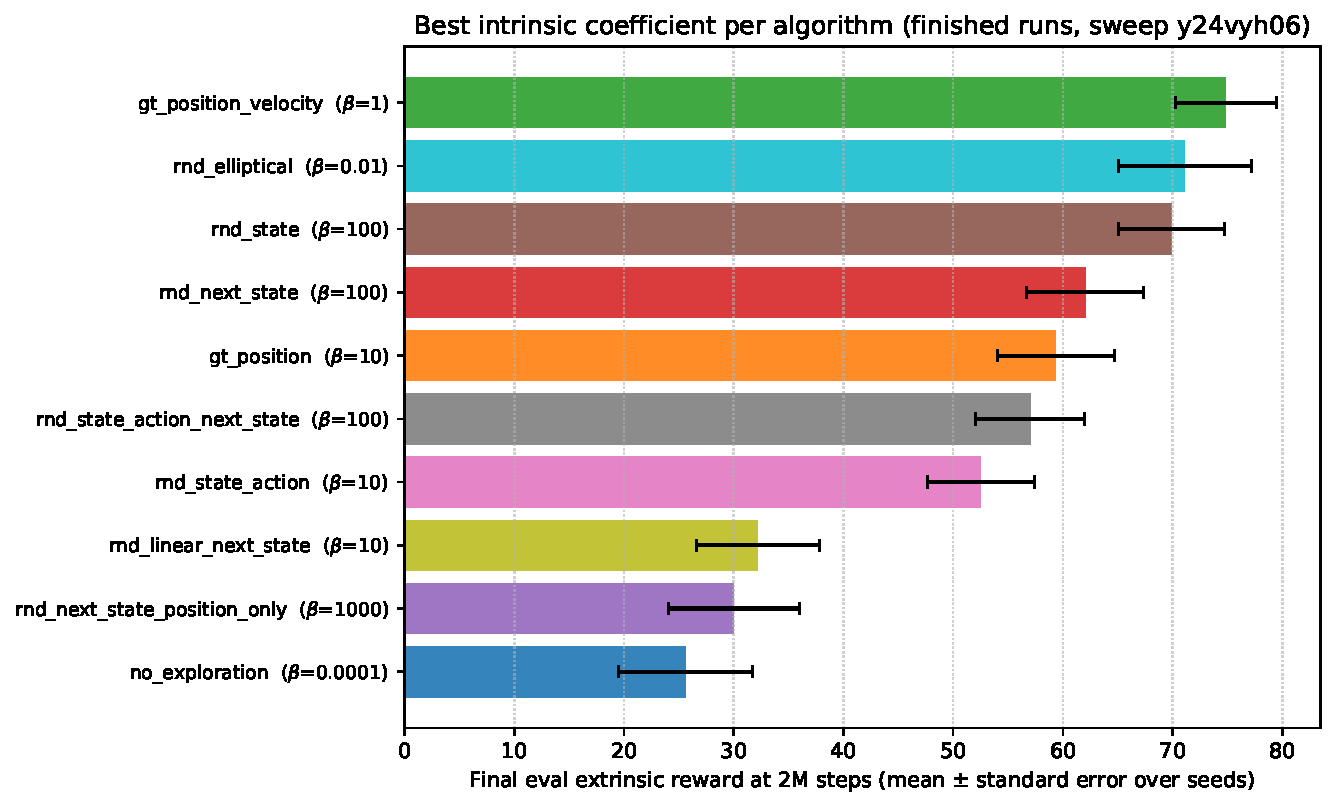
\includegraphics[width=0.86\linewidth]{../train_runs/2026-06-24-17-31_run_1_before_reorganization/analysis/plots/bar_best_beta_eval_reward.pdf}
\caption{Train run~1: final eval extrinsic reward $\bar{R}$ at $2\times10^{6}$ steps
for each algorithm at its best coefficient $\beta^\star$ (the $\beta$ in
parentheses), mean $\pm$ standard error over finished seeds. Bars are colored per
algorithm and sorted best-first; the same colors are used in
Figure~\ref{fig:trainrun1-curve}.}
\label{fig:trainrun1-bar}
\end{figure}

\paragraph{Learning curves.}
Figure~\ref{fig:trainrun1-curve} shows, for each algorithm's best-$\beta^\star$
group, the eval extrinsic reward as a function of training step (mean over seeds,
shaded band $=$ standard error). The ranking at $2\times10^{6}$ steps matches
Table~\ref{tab:trainrun1-best}; the count oracle and the elliptical bonus separate
from the rest by roughly $10^{6}$ steps.

\begin{figure}[H]
\centering
% Plot produced by ../train_runs/2026-06-24-17-31_run_1_before_reorganization/analysis/code/04_line_plot.py
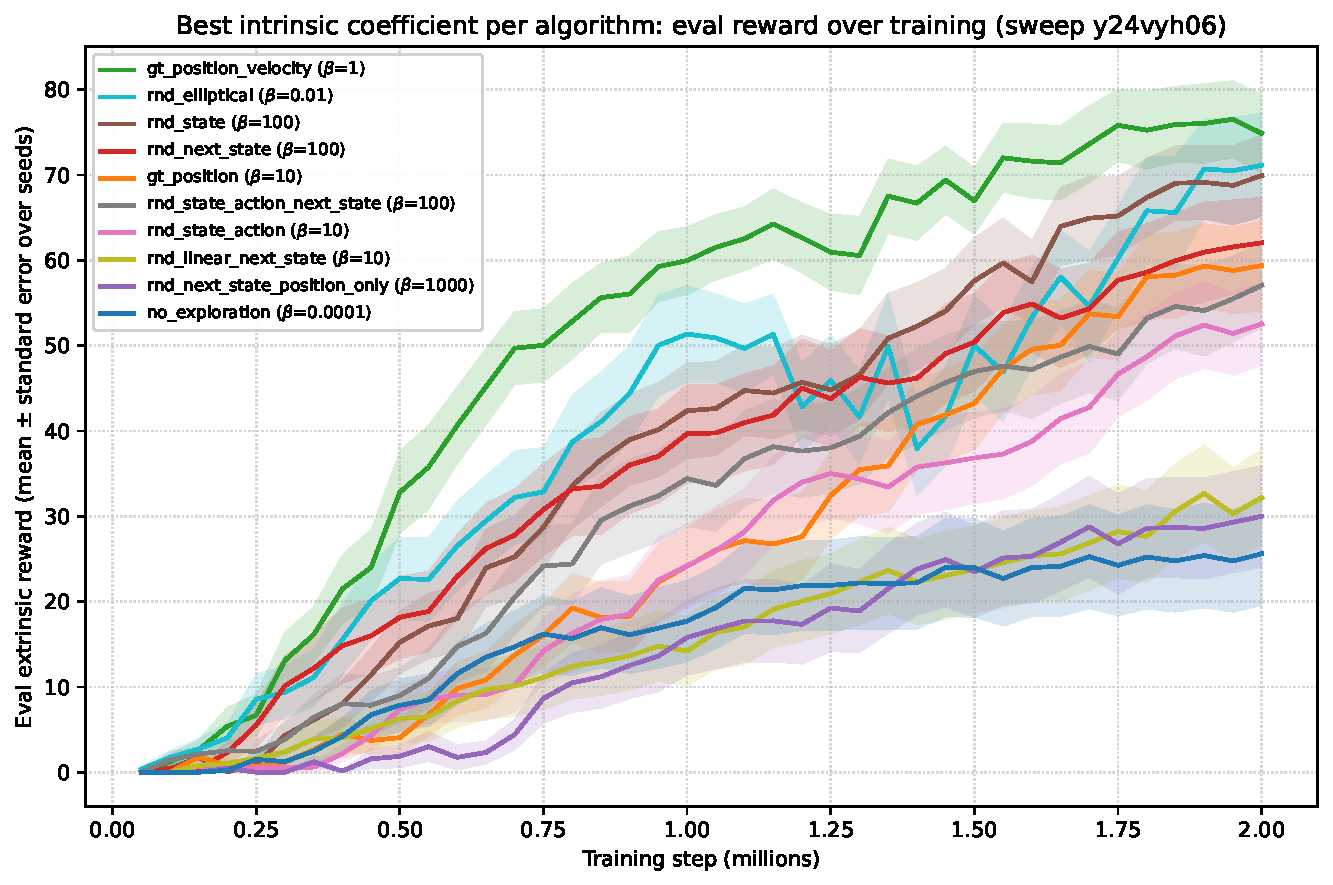
\includegraphics[width=0.92\linewidth]{../train_runs/2026-06-24-17-31_run_1_before_reorganization/analysis/plots/line_best_beta_eval_curve.pdf}
\caption{Train run~1: eval extrinsic reward over training for each algorithm at its
best coefficient $\beta^\star$. Each line is the seed mean of the best-$\beta^\star$
group; the shaded band is $\pm$ standard error over seeds. Colors match
Figure~\ref{fig:trainrun1-bar}; the legend is ordered by final reward.}
\label{fig:trainrun1-curve}
\end{figure}


\subsection{Train run 2 (after reorganization)}
\label{sec:train-run-2}

\paragraph{Run.}
Train run~2 re-runs the three best-performing methods of Train run~1 at their best-tuned intrinsic
coefficients on the reorganized \texttt{07\_reconstruction} package, with the fixed \texttt{top\_right}
goal. It is \textcolor{blue}{not a Weights \& Biases sweep}: configurations are handed out by a
\textcolor{blue}{local file work queue} and each run logs \textcolor{blue}{only to local JSON
(\texttt{use\_wandb}=False)}, so no run contacts wandb. The fixed (non-swept) hyperparameters are in
Table~\ref{tab:trainrun2-fixed} and the axes in Table~\ref{tab:trainrun2-sweep}; they match the run-1
configuration except for the values in \textcolor{blue}{blue} (\textcolor{blue}{$10^{6}$} training steps,
a \textcolor{blue}{$100$}-episode final evaluation, the \textcolor{blue}{three-algorithm} subset, and up
to \textcolor{blue}{$200$} seeds per algorithm). The run was \emph{cancelled after $312$ of the planned
$600$ runs had finished}; every table below states $n$, the number of finished seeds it pools, per
algorithm ($n=97$ for \texttt{gt\_\allowbreak position\_\allowbreak velocity}, $116$ for
\texttt{rnd\_\allowbreak elliptical}, $99$ for \texttt{rnd\_\allowbreak state}). The cancellation and how
to resume the remaining $288$ runs are recorded in the run folder's \texttt{CANCELLATION\_\allowbreak
AND\_\allowbreak RESUME.md}.

% Fixed (non-swept) hyperparameters of train run 2 — hand-authored static config; blue = differs from run 1.
\begin{table}[H]
\centering
\footnotesize
\setlength{\tabcolsep}{5pt}
\renewcommand{\arraystretch}{1.2}
\begin{tabular}{@{}>{\raggedright\arraybackslash}p{4.0cm} >{\raggedright\arraybackslash}p{4.6cm} >{\raggedright\arraybackslash}p{3.9cm}@{}}
\toprule
\textbf{Hyperparameter} & \textbf{Symbol} & \textbf{Value} \\
\midrule
Environment & \texttt{env\_name} & \texttt{PointMaze\_Large-v3} \\
Goal corner & \texttt{goal\_position} & \textcolor{blue}{\texttt{top\_right}} \\
Continuing task & \texttt{continuing\_task} & True \\
Reset target on goal & \texttt{reset\_target} & False \\
Max episode steps & \texttt{env\_max\_episode} & $400$ \\
Time-limit $\to$ termination & \texttt{apply\_\allowbreak termination\_\allowbreak wrapper} & False \\
\midrule
Training steps & \texttt{total\_timesteps} & \textcolor{blue}{$1\times10^{6}$} \\
Discount factor & $\gamma$ & $0.999$ \\
Policy / agent & --- & SAC (\texttt{MlpPolicy}) \\
Compute device & \texttt{device} & \texttt{cpu} \\
Evaluation frequency & \texttt{eval\_freq} & every $50000$ steps \\
Eval episodes (mid-training) & \texttt{n\_eval\_episodes} & $100$ \\
Eval episodes (final) & \texttt{n\_eval\_\allowbreak episodes\_\allowbreak final} & \textcolor{blue}{$100$} \\
\midrule
RND input normalization & \texttt{rnd\_obs\_norm} & True \\
RND distance & \texttt{rnd\_distance} & \texttt{mse} \\
RND output dimension & $m$ & $128$ \\
RND ensemble size & $N$ & $1$ \\
\bottomrule
\end{tabular}
\caption{Fixed (non-swept) hyperparameters of train run~2, held constant across the axes of
Table~\ref{tab:trainrun2-sweep}. Values match the run-1 configuration (Table~\ref{tab:trainrun1-fixed})
except those in \textcolor{blue}{blue}: the \texttt{top\_right} goal, $10^{6}$ training steps, and a
$100$-episode final evaluation.}
\label{tab:trainrun2-fixed}
\end{table}

\begin{table}[H]
\centering
\footnotesize
\setlength{\tabcolsep}{5pt}
\renewcommand{\arraystretch}{1.2}
\begin{tabular}{@{}>{\raggedright\arraybackslash}p{3.4cm} >{\raggedright\arraybackslash}p{2.1cm} >{\raggedright\arraybackslash}p{7.0cm}@{}}
\toprule
\textbf{Hyperparameter} & \textbf{Symbol} & \textbf{Values} \\
\midrule
Intrinsic-bonus method & \texttt{algorithm} & \textcolor{blue}{The three best methods of Train run~1}: \texttt{gt\_\allowbreak position\_\allowbreak velocity}, \texttt{rnd\_\allowbreak elliptical}, \texttt{rnd\_\allowbreak state}. \\
Intrinsic coefficient & $\beta$ & \textcolor{blue}{Pinned per algorithm to its run-1 $\beta^\star$}: \texttt{gt\_\allowbreak position\_\allowbreak velocity} $\beta{=}1$, \texttt{rnd\_\allowbreak elliptical} $\beta{=}0.01$, \texttt{rnd\_\allowbreak state} $\beta{=}100$ (not swept). \\
Random seed & \texttt{a\_seed} & \textcolor{blue}{$0$--$199$} ($200$ seeds; seeds \texttt{random}, \texttt{numpy}, \texttt{torch}, CUDA together). \\
Logging / dispatch & --- & \textcolor{blue}{Local file work queue; per-run JSON only, no wandb.} \\
\bottomrule
\end{tabular}
\caption{Axes of train run~2. Each algorithm is run at its single best-tuned coefficient $\beta^\star$
(from Table~\ref{tab:trainrun1-best}) across $200$ seeds; the grid is therefore
\texttt{algorithm} $\times$ \texttt{a\_seed} ($3\times200=600$ runs).}
\label{tab:trainrun2-sweep}
\end{table}

\paragraph{Aggregation.}
As in Train run~1, runs are grouped by algorithm (each at its single $\beta^\star$). The primary metric
is the final eval extrinsic reward $r^{\mathrm{ext}}$ (the \textcolor{blue}{$100$}-episode evaluation at
\textcolor{blue}{$10^{6}$} steps); for $n$ seeds with per-seed final rewards $R_i$ we report the seed mean
$\bar{R}$ and standard error $\mathrm{SE}=s/\sqrt{n}$ (as in Eq.~(1) of Train run~1).
Table~\ref{tab:trainrun2-best} lists $(\beta^\star,\bar{R},\mathrm{SE},n)$ per algorithm,
Figure~\ref{fig:trainrun2-bar} shows the same final rewards as bars, and Figure~\ref{fig:trainrun2-curve}
the eval reward over training. Table~\ref{tab:trainrun2-dist} gives the distance to the ground-truth
visit-count field.

\begin{table}[H]
\centering
\footnotesize
\setlength{\tabcolsep}{8pt}
\renewcommand{\arraystretch}{1.2}
% Train run 2 reward table (pooled over all finished seeds; single local logging mode, no wandb).
% Higher reward is better; rows sorted by Rbar descending; best bold, second-best underlined.
\begin{tabular}{@{}>{\raggedright\arraybackslash}p{4.6cm} r r r r@{}}
\toprule
\textbf{Algorithm} & \textbf{$\beta^\star$} & \textbf{$\bar{R}$ ($\downarrow$)} & \textbf{SE} & \textbf{$n$} \\
\midrule
\texttt{gt\_position\_velocity} & $1$ & \textbf{67.76} & 2.44 & 97 \\
\texttt{rnd\_elliptical} & $0.01$ & \underline{44.49} & 3.32 & 116 \\
\texttt{rnd\_state} & $100$ & 35.79 & 3.32 & 99 \\
\bottomrule
\end{tabular}

\caption{Train run~2: best-tuned coefficient $\beta^\star$ per algorithm with the final eval extrinsic
reward $\bar{R}$ (mean over $n$ finished seeds), its standard error, and $n$. Rows sorted by $\bar{R}$
descending; best \textbf{bold}, second \underline{underlined}; higher reward is better. The run was
cancelled at $312/600$ finished, so $n$ is the number of finished seeds pooled per algorithm.}
\label{tab:trainrun2-best}
\end{table}

\begin{figure}[H]
\centering
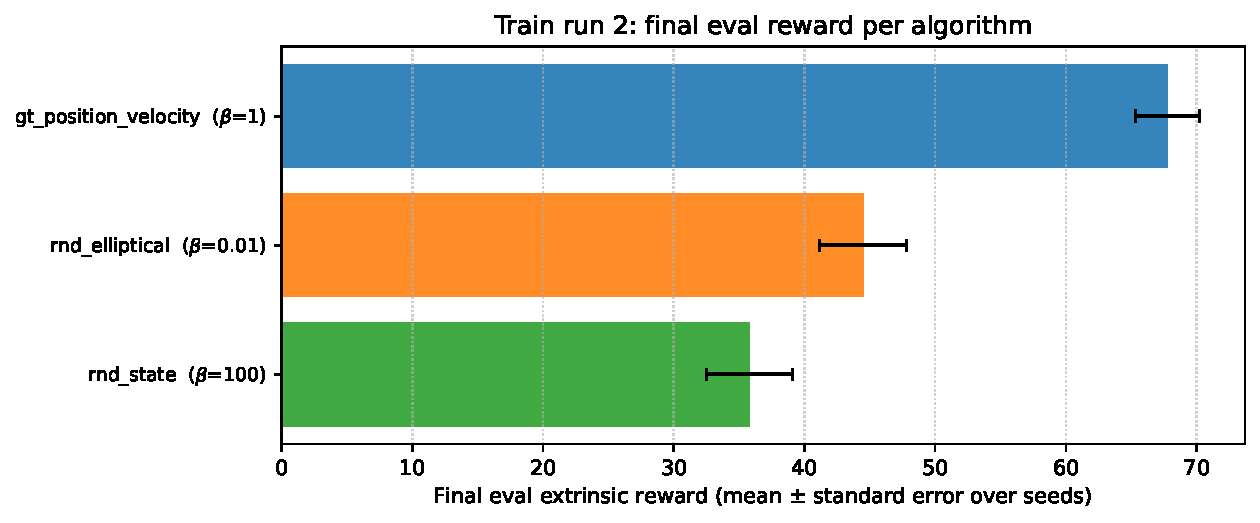
\includegraphics[width=0.86\linewidth]{../train_runs/2026-06-24-21-24_run_2_after_reorganization/analysis/plots/bar_final_reward.pdf}
\caption{Train run~2: final eval extrinsic reward $\bar{R}$ at \textcolor{blue}{$10^{6}$} steps per
algorithm (mean $\pm$ standard error over finished seeds), each at its $\beta^\star$. The
\textcolor{blue}{three-algorithm} subset of Train run~1, at \textcolor{blue}{$10^{6}$} steps.}
\label{fig:trainrun2-bar}
\end{figure}

\begin{figure}[H]
\centering
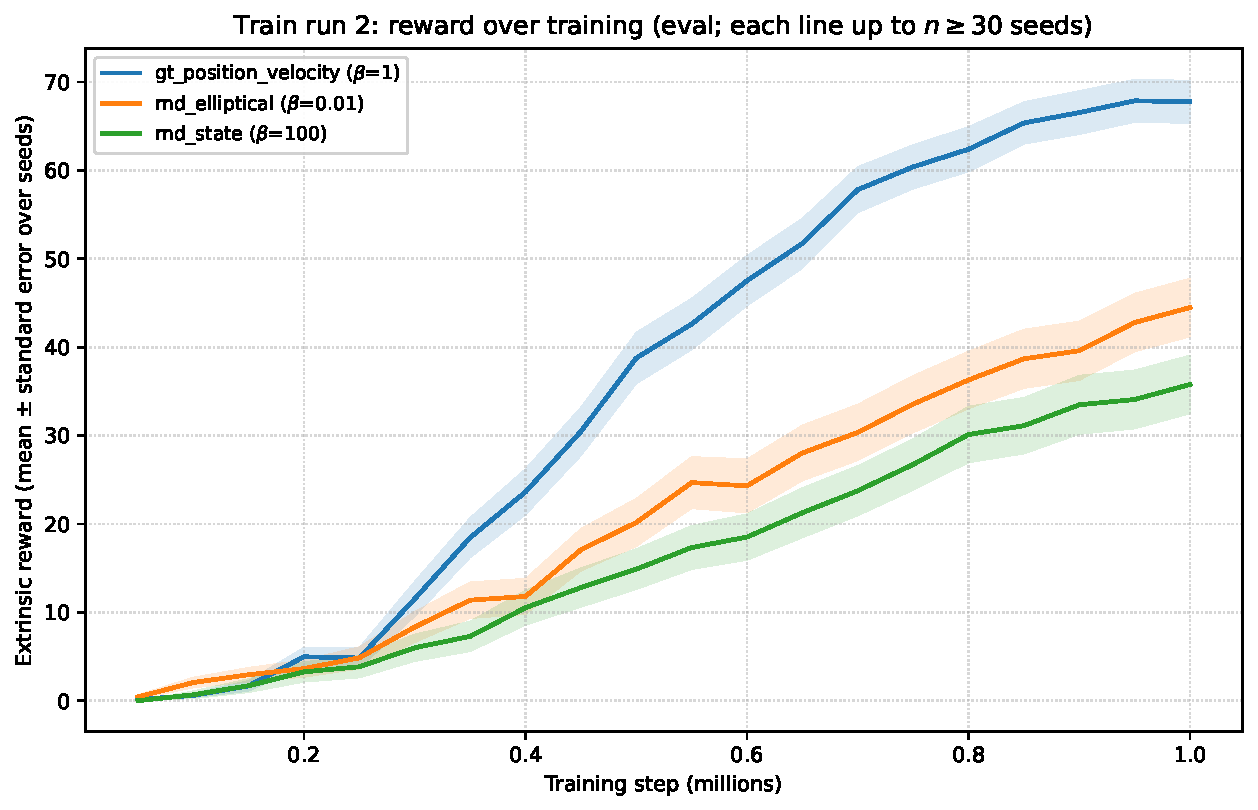
\includegraphics[width=0.92\linewidth]{../train_runs/2026-06-24-21-24_run_2_after_reorganization/analysis/plots/line_reward_curve.pdf}
\caption{Train run~2: eval extrinsic reward over training for each algorithm at its $\beta^\star$
(mean $\pm$ standard error over seeds). \textcolor{blue}{Each line is drawn only up to the largest step
reached by at least $30$ seeds}, so no plotted segment averages fewer than 30 runs.}
\label{fig:trainrun2-curve}
\end{figure}

\begin{table}[H]
\centering
\footnotesize
\setlength{\tabcolsep}{4pt}
\renewcommand{\arraystretch}{1.2}
% Train run 2 distance-to-ground-truth table (pooled over all finished seeds; single local mode, no wandb).
% Lower distance is better; rows sorted ascending by normalized_l2; per column best bold, second underlined.
\begin{tabular}{@{}>{\raggedright\arraybackslash}p{3.0cm} r r r r r r@{}}
\toprule
\textbf{Algorithm} & \textbf{\shortstack[r]{\texttt{min\_c\_}\\ \texttt{l1\_diff}}} & \textbf{\shortstack[r]{\texttt{min\_c\_}\\ \texttt{l2\_diff}}} & \textbf{\shortstack[r]{\texttt{min\_c\_}\\ \texttt{l1\_inv}}} & \textbf{\shortstack[r]{\texttt{min\_c\_}\\ \texttt{l2\_inv}}} & \textbf{\shortstack[r]{\texttt{normalized\_}\\ \texttt{l2} ($\uparrow$)}} & \textbf{\shortstack[r]{\texttt{normalized\_}\\ \texttt{angle\_rad}}} \\
\midrule
\texttt{gt\_position\_velocity} & \textbf{0.00114} & \textbf{0} & \textbf{2.88e-14} & \textbf{1.78e-15} & \textbf{0} & \textbf{2.76e-06} \\
\texttt{rnd\_state} & \underline{2.02e+03} & \underline{37.8} & \underline{2.32} & \underline{0.0692} & \underline{49} & \underline{0.733} \\
\bottomrule
\end{tabular}

\caption{Train run~2: distance between each algorithm's learned intrinsic-bonus field and the oracle
\texttt{gt\_position\_velocity} visit-count field (lower is better; per column, best \textbf{bold},
second \underline{underlined}). Only algorithms whose bonus is a per-cell field over the maze, comparable
to the visit-count oracle, are listed: \texttt{gt\_position\_velocity} (the oracle itself, $\approx 0$)
and \texttt{rnd\_state}. \textcolor{blue}{\texttt{rnd\_elliptical} is omitted} --- its elliptical bonus is
not in \texttt{ALGORITHMS\_NO\_ACTION}, so no distance-to-ground-truth field is logged for it.}
\label{tab:trainrun2-dist}
\end{table}

\subsection{Train run 3 (proposed): cumulative elliptical bonuses and count-aware RND optimizers}
\label{sec:train-run-3-proposed}

\paragraph{Purpose.}
Train run~1 showed that the count oracle \texttt{gt\_position\_velocity} is the
best method and that the learned \texttt{rnd\_elliptical} bonus is the closest
learned competitor. The next run should not merely repeat the same sweep. It
should test the two mechanisms that the previous sections identify as most
important:
\begin{enumerate}[leftmargin=1.4em,itemsep=2pt,topsep=2pt]
\item whether the elliptical bonus should use a per-batch covariance
$\Lambda_B$ or a cumulative covariance $\Lambda_t$;
\item whether RND predictors need count-aware optimizers instead of constant-rate
Adam.
\end{enumerate}

\paragraph{Main hypotheses.}
The proposed run tests four hypotheses.
\begin{description}[leftmargin=1.8em,itemsep=2pt,topsep=2pt]
\item[H1.]
A cumulative elliptical matrix
\[
\Lambda_t=\lambda I+\sum_{\tau\le t}\varphi_\tau\varphi_\tau^\top
\]
will produce a more count-like bonus than the current per-batch matrix
\[
\Lambda_B=\frac1b\Phi_B^\top\Phi_B+\lambda I.
\]

\item[H2.]
If \texttt{rnd\_elliptical} is strong because it approximates the count oracle,
then the cumulative version should improve the distance-to-ground-truth metrics
of Section~\ref{sec:metrics}, especially the normalized-angle and scale-fit
metrics between the prediction field $p$ and the ground-truth field $g$.

\item[H3.]
For RND predictors, replacing constant-rate Adam with a count-aware optimizer
such as AdaGrad, SGD with $\eta_t=\eta_0/(t+t_0)$, or Polyak--Ruppert averaging
should reduce late-training bonus saturation.

\item[H4.]
The L2 residual readout
\[
\lVert g_\phi(\tilde{x})-f_\theta(\tilde{x})\rVert_2
\]
should match the count oracle's $1/\sqrt{n}$ scale better than the default
squared-error readout
\[
\frac12\lVert g_\phi(\tilde{x})-f_\theta(\tilde{x})\rVert_2^2.
\]
\end{description}

\paragraph{Fixed training setup.}
Use the same base training configuration as Section~\ref{sec:env-loop}: SAC with
\texttt{MlpPolicy}, \texttt{PointMaze\_Large-v3}, $2\times 10^6$ training steps,
discount factor $\gamma=0.999$, evaluation every $50000$ steps, $100$ evaluation
episodes during training, and $10^4$ final evaluation episodes. Since the project
has been reorganized after Train run~1, use the current fixed goal convention
\[
\texttt{goal\_position}=\texttt{top\_right}
\]
for this run.

\paragraph{Two-stage design.}
The proposed run has two stages. Stage A is a cheaper diagnostic stage that checks
whether the bonus has the right shape. Stage B is the full SAC training stage that
checks whether the better-shaped bonus actually improves control.

\paragraph{Stage A: bonus-shape diagnostic before full SAC.}
Before launching the full grid, run every candidate bonus on the same saved replay
stream. This removes policy feedback and asks a cleaner question: given the same
visited data, does the method produce a count-like field?

For each candidate, evaluate the prediction field $p$ on the grid $G$ and compare
it to the oracle field $g$ using the existing metrics of Section~\ref{sec:metrics}.
Also estimate the empirical decay slope of the bonus with respect to visit count.
For grid cells indexed by $i$, let $n_i$ be the oracle visit count and $p_i$ the
candidate bonus. Fit
\begin{align}
(\widehat{c},\widehat{\alpha}_{\mathrm{bonus}})
=
\argmin_{c,\alpha}
\sum_{i\in G}
\left[
\log(p_i+\varepsilon)
-
c
-
\alpha\log(n_i+1)
\right]^2.
\end{align}
A count-like L2 bonus should have
\[
\widehat{\alpha}_{\mathrm{bonus}}\approx -\frac12.
\]
A squared-error RND bonus should be expected to have a slope closer to $-1$ if the
underlying residual norm is count-like.

\paragraph{Probe field for action-conditioned bonuses.}
The current distance-to-ground-truth logging skips action-conditioned methods
because $g$ is defined over the state grid $G$, while methods such as
\texttt{rnd\_elliptical} depend on $a$. For Train run~3, log a probe field by
averaging over a small fixed action set:
\begin{align}
A_{\mathrm{probe}}
=
\{(0,0),(1,0),(-1,0),(0,1),(0,-1)\}.
\end{align}
For a grid state $s_i\in G$, define
\begin{align}
p_i^{\mathrm{probe}}
=
\frac{1}{|A_{\mathrm{probe}}|}
\sum_{a\in A_{\mathrm{probe}}}
r^{\mathrm{int}}(s_i,a).
\end{align}
Then use $p^{\mathrm{probe}}$ in the same distance metrics that compare $p$ to
$g$. This lets us evaluate action-conditioned methods instead of skipping them.

\paragraph{Stage B: full SAC sweep.}
After Stage A, run the full SAC sweep on the candidates in
Table~\ref{tab:trainrun3-candidates}. Keep the two oracle baselines and the
current best learned methods as controls. The purpose is to isolate mechanism,
not only to maximize reward.

\begin{table}[H]
\centering
\footnotesize
\setlength{\tabcolsep}{3.5pt}
\renewcommand{\arraystretch}{1.25}
\begin{tabular}{@{}>{\raggedright\arraybackslash}p{2.5cm} >{\raggedright\arraybackslash}p{3.7cm} >{\raggedright\arraybackslash}p{5.3cm}@{}}
\toprule
\textbf{Class} & \textbf{Candidate} & \textbf{What it tests} \\
\midrule
Baseline &
\texttt{no\_\allowbreak exploration} &
SAC without intrinsic reward; verifies the task difficulty. \\
\midrule
Oracle count &
\texttt{gt\_\allowbreak position\_\allowbreak velocity} &
Upper reference: true count field $g$ over position and velocity. \\
\midrule
Oracle count &
\texttt{gt\_\allowbreak position} &
Simpler count reference: position-only counting. \\
\midrule
Current learned control &
\texttt{rnd\_\allowbreak elliptical} &
The current per-batch elliptical method from Train run~1. \\
\midrule
Elliptical &
\texttt{elliptical\_\allowbreak cumulative\_\allowbreak sa} &
Replace $\Lambda_B$ with cumulative $\Lambda_t$ using features of $[s;a]$. \\
\midrule
Elliptical &
\texttt{elliptical\_\allowbreak discounted\_\allowbreak sa} &
Use discounted cumulative memory with $\rho_\Lambda<1$ to test whether old data
should gradually fade. \\
\midrule
Elliptical &
\texttt{elliptical\_\allowbreak cumulative\_\allowbreak state} &
Use cumulative random features of $s$ only; action-free, so $p$ can be compared
directly to $g$. \\
\midrule
Elliptical &
\texttt{elliptical\_\allowbreak cumulative\_\allowbreak next\_\allowbreak state} &
Use cumulative random features of $s'$ only; tests whether next-state novelty is
better aligned with the count oracle. \\
\midrule
Current RND control &
\texttt{rnd\_\allowbreak next\_\allowbreak state\_\allowbreak adam\_\allowbreak mse} &
Current RND style: Adam optimizer and squared-error bonus. \\
\midrule
Optimizer &
\texttt{rnd\_\allowbreak next\_\allowbreak state\_\allowbreak adam\_\allowbreak l2} &
Keeps Adam but changes readout from squared error to L2 residual; isolates the
effect of the bonus scale. \\
\midrule
Optimizer &
\texttt{rnd\_\allowbreak next\_\allowbreak state\_\allowbreak adagrad\_\allowbreak l2} &
Tests whether cumulative adaptive steps reduce saturation for ordinary RND. \\
\midrule
Optimizer &
\texttt{rnd\_\allowbreak linear\_\allowbreak next\_\allowbreak state\_\allowbreak adagrad\_\allowbreak l2} &
Tests the cleanest match between fixed random features, a linear predictor, a
count-aware optimizer, and L2 readout. \\
\midrule
Optimizer &
\texttt{rnd\_\allowbreak linear\_\allowbreak next\_\allowbreak state\_\allowbreak sgd1t\_\allowbreak l2} &
Tests the explicit $\eta_t=\eta_0/(t+t_0)$ schedule predicted to give
$1/\sqrt{n}$ residual decay. \\
\midrule
Optimizer &
\texttt{rnd\_\allowbreak linear\_\allowbreak next\_\allowbreak state\_\allowbreak polyak\_\allowbreak l2} &
Tests Polyak--Ruppert averaging of the linear RND predictor. \\
\bottomrule
\end{tabular}
\caption{Candidate methods for Train run~3. The elliptical block tests whether
the feature covariance should accumulate across training. The optimizer block
tests whether RND needs count-aware optimization and L2 residual readout.}
\label{tab:trainrun3-candidates}
\end{table}

\paragraph{Swept hyperparameters.}
Use a smaller but still logarithmic $\beta$ sweep for the pilot, then expand only
the best candidates. The recommended pilot grid is
\begin{align}
\beta
\in
\{10^{-3},10^{-2},10^{-1},1,10,10^2\}.
\end{align}
For final confirmation, add the endpoints from Train run~1:
\[
\beta\in\{10^{-4},10^{-3},10^{-2},10^{-1},1,10,10^2,10^3\}.
\]

For the new elliptical methods, sweep the regularizer
\[
\lambda\in\{10^{-6},10^{-4},10^{-2}\}
\]
in Stage A. In full SAC, keep only the best $\lambda$ per elliptical method from
Stage A, unless the Stage A curves show that performance is highly sensitive to
$\lambda$.

For discounted cumulative elliptical, sweep
\[
\rho_\Lambda\in\{0.99,0.999,1.0\},
\]
where $\rho_\Lambda=1.0$ is the ordinary cumulative version.

For optimizer methods, use the following pilot settings:
\begin{align}
\eta
&\in
\{10^{-4},10^{-3}\}
\quad\text{for Adam and AdaGrad},\\
\eta_0
&\in
\{10^{-2},10^{-1},1\},
\qquad
t_0\in\{10^3,10^4\}
\quad\text{for SGD with } \eta_t=\eta_0/(t+t_0).
\end{align}
The final SAC sweep should keep only the optimizer learning-rate setting that
wins the Stage A bonus-shape diagnostic.

\begin{table}[H]
\centering
\footnotesize
\setlength{\tabcolsep}{4pt}
\renewcommand{\arraystretch}{1.25}
\begin{tabular}{@{}>{\raggedright\arraybackslash}p{3.2cm} >{\raggedright\arraybackslash}p{3.8cm} >{\raggedright\arraybackslash}p{4.8cm}@{}}
\toprule
\textbf{Axis} & \textbf{Pilot values} & \textbf{Reason} \\
\midrule
Intrinsic coefficient $\beta$ &
$\{10^{-3},10^{-2},10^{-1},1,10,10^2\}$ &
Covers the useful range around the best Train run~1 values without the full cost. \\
\midrule
Elliptical regularizer $\lambda$ &
$\{10^{-6},10^{-4},10^{-2}\}$ &
Tests whether the inverse covariance is too sharp or too smooth. \\
\midrule
Discount factor for $\Lambda_t$ &
$\rho_\Lambda\in\{0.99,0.999,1.0\}$ &
Tests recent-memory versus full-memory feature counts. \\
\midrule
Optimizer learning rate $\eta$ &
$\{10^{-4},10^{-3}\}$ &
Covers the common RND learning-rate range. \\
\midrule
SGD schedule constants &
$\eta_0\in\{10^{-2},10^{-1},1\}$, $t_0\in\{10^3,10^4\}$ &
Controls how fast the $1/t$ optimizer becomes conservative. \\
\midrule
Random seeds \texttt{a\_seed} &
$0$--$29$ pilot; $0$--$99$ confirmation &
Pilot identifies promising methods; confirmation reduces seed noise. \\
\bottomrule
\end{tabular}
\caption{Recommended swept axes for Train run~3. The pilot should be used to
select mechanisms; the confirmation run should use the full seed set only for the
best candidates.}
\label{tab:trainrun3-sweep}
\end{table}

\paragraph{Primary metrics.}
The primary control metric remains final evaluation extrinsic reward:
\[
\bar{R}
=
\frac1n\sum_{i=1}^{n}R_i,
\qquad
\mathrm{SE}
=
\frac{s}{\sqrt{n}}.
\]
As in Train run~1, select the best coefficient
\[
\beta^\star
=
\argmax_{\beta}
\bar{R}(\texttt{algorithm},\beta)
\]
for each algorithm.

\paragraph{Secondary diagnostic metrics.}
In addition to final reward, log the following diagnostics:
\begin{enumerate}[leftmargin=1.4em,itemsep=2pt,topsep=2pt]
\item all distance-to-ground-truth metrics from Section~\ref{sec:metrics};
\item the bonus-count slope $\widehat{\alpha}_{\mathrm{bonus}}$;
\item the median intrinsic bonus in low-count, medium-count, and high-count cells;
\item the saturation ratio
\[
S_{\mathrm{sat}}
=
\frac{
\mathrm{median}\{p_i:\,n_i\text{ is in the top count quartile}\}
}{
\mathrm{median}\{p_i:\,n_i\text{ is in the bottom count quartile}\}
+\varepsilon
};
\]
\item for elliptical methods, $\log\det(\Lambda_t)$ or
$\sum_j\log(\ell_j)$, which measures how much feature space has been covered;
\item for RND methods, the mean L2 residual
\[
\frac1{|G|}\sum_{s_i\in G}
\lVert g_\phi(\tilde{s}_i)-f_\theta(\tilde{s}_i)\rVert_2
\]
and the mean squared residual
\[
\frac1{|G|}\sum_{s_i\in G}
\frac12
\lVert g_\phi(\tilde{s}_i)-f_\theta(\tilde{s}_i)\rVert_2^2.
\]
\end{enumerate}

\paragraph{Decision rules.}
The next run should answer the following concrete questions.

\begin{enumerate}[leftmargin=1.4em,itemsep=2pt,topsep=2pt]
\item \textbf{Does cumulative elliptical improve the bonus shape?}
It succeeds if its distance to $g$ is lower than the current per-batch
\texttt{rnd\_elliptical} distance, and if
\[
\widehat{\alpha}_{\mathrm{bonus}}
\]
is closer to $-1/2$.

\item \textbf{Does cumulative elliptical improve control?}
It succeeds as an RL method if its best-$\beta^\star$ final reward $\bar{R}$ is
higher than or statistically comparable to the current \texttt{rnd\_elliptical}
while also having better bonus-shape diagnostics.

\item \textbf{Does action conditioning matter?}
Compare \texttt{elliptical\_cumulative\_sa} against
\texttt{elliptical\_cumulative\_state} and
\texttt{elliptical\_cumulative\_next\_state}. If the state-only methods match
$g$ better but the state-action method gets higher reward, then action novelty is
useful even when it is not fully captured by the state-only ground-truth field.

\item \textbf{Does optimizer choice matter for RND?}
AdaGrad, $1/t$ SGD, or Polyak averaging succeeds if it reduces late-stage
saturation and gives a bonus-count slope closer to the target scale than
constant-rate Adam.

\item \textbf{Does readout scale matter?}
If \texttt{rnd\_next\_state\_adam\_l2} has better count-like diagnostics than
\texttt{rnd\_next\_state\_adam\_mse}, then the mismatch is partly the squared-error
readout, not only the optimizer.
\end{enumerate}

\paragraph{Expected result.}
The most likely outcome is that cumulative elliptical will give the cleanest
count-like bonus because it explicitly stores a running feature count through
$\Lambda_t$. Among optimizer methods, the strongest candidate is
\texttt{rnd\_linear\_next\_state\_adagrad\_l2}, because it combines fixed random
features, a linear predictor, a cumulative optimizer, and an L2 residual readout.
If these diagnostics improve but final SAC reward does not, then the limiting
factor is probably not the mathematical count approximation itself, but how the
intrinsic reward changes the policy's data distribution.

\clearpage
\bibliographystyle{plainnat}
\bibliography{bibliography}

\clearpage
\appendix

\section{Distance to ground truth metrics}
\label{sec:metrics}

Each metric compares a method's bonus field $p$ to the oracle field $g$ over the grid
$G$ and returns a single scalar distance $D$ (logged as \texttt{distance\_to\_gt/*}).
Distance is only logged for methods whose bonus field can be built without actions
(\texttt{no\_exploration}, the two count methods, \texttt{rnd\_next\_state},
\texttt{rnd\_next\_state\_position\_only}, \texttt{rnd\_state},
\texttt{rnd\_linear\_next\_state}); action-conditioned methods are skipped.
Table~\ref{tab:metrics} summarizes the six metrics; the three families are detailed below.

\begin{table}[H]
\centering
\footnotesize
\setlength{\tabcolsep}{4pt}
\renewcommand{\arraystretch}{1.25}
\begin{tabular}{@{}>{\raggedright\arraybackslash}p{2.4cm} >{\raggedright\arraybackslash}p{2.7cm} >{\raggedright\arraybackslash}p{3.0cm} >{\raggedright\arraybackslash}p{4.0cm}@{}}
\toprule
\textbf{Family} & \textbf{Metric} & \textbf{Formula} & \textbf{What it measures} \\
\midrule
\multirow{2}{2.4cm}{Scale-fit} & \texttt{min\_c\_l1\_diff} & $\min_c\lVert g-c\,p\rVert_1$ & Best-scaled $L_1$ mismatch to the GT field. \\
 & \texttt{min\_c\_l2\_diff} & $\min_c\lVert g-c\,p\rVert_2$ & Best-scaled $L_2$ mismatch (closed-form $c$). \\
\midrule
\multirow{2}{2.4cm}{Inverse-ratio} & \texttt{min\_c\_l1\_inv} & $\min_c\lVert c\mathbf{1}-z\rVert_1$ & $L_1$ spread of the ratio $z=p\oslash g$ ($c^\star=\mathrm{median}$). \\
 & \texttt{min\_c\_l2\_inv} & $\min_c\lVert c\mathbf{1}-z\rVert_2$ & $L_2$ spread of the ratio $z$ ($c^\star=\mathrm{mean}$). \\
\midrule
\multirow{2}{2.4cm}{Normalized geometry} & \texttt{normalized\_l2} & $\lVert\hat{g}-\hat{p}\rVert_2$ & $L_2$ distance after max-absolute scaling. \\
 & \texttt{normalized\_\allowbreak angle\_\allowbreak rad} & $\arccos\langle u_g,u_p\rangle$ & Angle between unit vectors, in $[0,\pi]$. \\
\bottomrule
\end{tabular}
\caption{Distance-to-ground-truth metrics: each compares a method's bonus field $p$ to the
oracle field $g$ over the grid $G$ and returns a scalar distance $D$. The symbols $z$,
$\hat{g}$, $\hat{p}$, $u_g$, $u_p$ are defined in the respective subsections below.}
\label{tab:metrics}
\end{table}

\subsection{Scale-fit metrics}
\label{sec:dist-scale}

The scale-fit family is invariant to the overall magnitude of $p$: it fits a single
scalar $c$ and reports the residual, $D = \min_{c}\lVert g - c\,p\rVert$.

\paragraph{\texttt{min\_c\_l1\_diff}.}
\begin{align}
D = \min_{c}\lVert g - c\,p\rVert_1 = \min_c\sum_i|g_i - c\,p_i|,
\end{align}
with $c$ found by bounded 1-D numerical search. An exact minimizer is in fact available: $c^\star$ is the weighted median of the ratios $g_i/p_i$ with weights $|p_i|$ (the $L_1$ counterpart of the $L_2$ projection above), so the numerical search is a convenience, not a necessity. If $p\equiv0$, $D = \lVert g\rVert_1$.

\paragraph{\texttt{min\_c\_l2\_diff}.}
Closed-form least-squares scale:
\begin{align}
D = \lVert g - c^\star p\rVert_2, \qquad c^\star = \frac{\langle g,p\rangle}{\langle p,p\rangle}.
\end{align}
\emph{Why this $c^\star$.} It is the minimizer of $\min_c\lVert g-c\,p\rVert_2$: the squared objective $f(c)=\lVert g-c\,p\rVert_2^2=\langle g,g\rangle-2c\,\langle g,p\rangle+c^2\langle p,p\rangle$ is a convex quadratic in the scalar $c$, so its stationary point $f'(c)=-2\langle g,p\rangle+2c\,\langle p,p\rangle=0$---that is, $c^\star=\langle g,p\rangle/\langle p,p\rangle$---is the global minimum (the quadratic opens upward because $\langle p,p\rangle\ge0$). If $p\equiv0$, $D = \lVert g\rVert_2$.

\subsection{Inverse-ratio metrics}
\label{sec:dist-inv}

These ask whether $p$ is a single constant multiple of $g$ \emph{cell by cell}. Form the
element-wise ratio $z = p \oslash g$ (with $g$ regularized so $|g_i|\ge\varepsilon=10^{-8}$,
sign preserved), fit one constant $c$, and report $D = \min_{c}\lVert c\mathbf{1} - z\rVert$.
A small value means $p/g$ is nearly constant across all cells.

\paragraph{\texttt{min\_c\_l1\_inv}.}
The $L_1$ minimizer is the median:
\begin{align}
D = \sum_i|c^\star - z_i|, \qquad c^\star = \mathrm{median}(z).
\end{align}

\paragraph{\texttt{min\_c\_l2\_inv}.}
The $L_2$ minimizer is the mean:
\begin{align}
D = \lVert c^\star\mathbf{1} - z\rVert_2, \qquad c^\star = \bar{z}.
\end{align}
Equivalent to $\sqrt{n}$ times the standard deviation of $z$.

\subsection{Normalized-geometry metrics}
\label{sec:dist-norm}

Rescale both vectors to a common scale, then compare their shape. One uses max-absolute
scaling and an $L_2$ difference; the other compares directions via the angle between unit
vectors.

\paragraph{\texttt{normalized\_l2}.}
\begin{align}
D = \Big\lVert \frac{g}{\max_i|g_i|+\varepsilon} - \frac{p}{\max_i|p_i|+\varepsilon}\Big\rVert_2,
\end{align}
with $\varepsilon=10^{-10}$ (each vector's peak magnitude scaled to $\approx1$).

\paragraph{\texttt{normalized\_angle\_rad}.}
\begin{align}
D = \arccos\!\big(\mathrm{clip}(\langle u_g, u_p\rangle, -1, 1)\big)\in[0,\pi],
\end{align}
where $u_g = g/(\lVert g\rVert_2+\varepsilon)$ and $u_p = p/(\lVert p\rVert_2+\varepsilon)$
are the unit directions ($\varepsilon=10^{-10}$). $0$ = same direction, $\pi$ = opposite.


\subsection{Metric applicability by algorithm}
\label{sec:metric-applicability}

Not every algorithm yields a bonus field that can be compared to the oracle, so not every
metric can be computed for every algorithm. Table~\ref{tab:metric-applicability} marks, for
each of the ten \texttt{--algorithm} choices, which of the six distance metrics are computed
(\ding{51}; a blank cell means the metric is not computed for that algorithm). The split is
decided per algorithm rather than per metric: the dispatcher
(\texttt{compute\_intrinsic\_vector\_distance}) computes \emph{all six} metrics for an
algorithm whose bonus is a function of the state (or next state) alone, and \emph{none} for an
action-conditioned algorithm (it returns nothing, so \texttt{distance\_to\_gt/*} is never
logged). The reason for each algorithm is enumerated below.

\begin{table}[H]
\centering
\scriptsize
\setlength{\tabcolsep}{3pt}
\renewcommand{\arraystretch}{1.15}
\resizebox{\textwidth}{!}{%
\begin{tabular}{@{}l
  >{\centering\arraybackslash}p{1.5cm}
  >{\centering\arraybackslash}p{1.1cm}
  >{\centering\arraybackslash}p{1.25cm}
  >{\centering\arraybackslash}p{0.9cm}
  >{\centering\arraybackslash}p{1.25cm}
  >{\centering\arraybackslash}p{0.9cm}
  >{\centering\arraybackslash}p{1.05cm} |
  >{\centering\arraybackslash}p{1.0cm}
  >{\centering\arraybackslash}p{1.05cm}
  >{\centering\arraybackslash}p{1.35cm}@{}}
\toprule
 & \texttt{no\_\allowbreak exploration}
 & \texttt{gt\_\allowbreak position}
 & \texttt{gt\_\allowbreak position\_\allowbreak velocity}
 & \texttt{rnd\_\allowbreak next\_\allowbreak state}
 & \texttt{rnd\_\allowbreak next\_\allowbreak state\_\allowbreak position\_\allowbreak only}
 & \texttt{rnd\_\allowbreak state}
 & \texttt{rnd\_\allowbreak linear\_\allowbreak next\_\allowbreak state}
 & \texttt{rnd\_\allowbreak state\_\allowbreak action}
 & \texttt{rnd\_\allowbreak state\_\allowbreak action\_\allowbreak next\_\allowbreak state}
 & \texttt{rnd\_\allowbreak elliptical} \\
\midrule
\texttt{min\_c\_l1\_diff}       & \ding{51} & \ding{51} & \ding{51} & \ding{51} & \ding{51} & \ding{51} & \ding{51} &  &  &  \\
\texttt{min\_c\_l2\_diff}       & \ding{51} & \ding{51} & \ding{51} & \ding{51} & \ding{51} & \ding{51} & \ding{51} &  &  &  \\
\texttt{min\_c\_l1\_inv}        & \ding{51} & \ding{51} & \ding{51} & \ding{51} & \ding{51} & \ding{51} & \ding{51} &  &  &  \\
\texttt{min\_c\_l2\_inv}        & \ding{51} & \ding{51} & \ding{51} & \ding{51} & \ding{51} & \ding{51} & \ding{51} &  &  &  \\
\texttt{normalized\_l2}         & \ding{51} & \ding{51} & \ding{51} & \ding{51} & \ding{51} & \ding{51} & \ding{51} &  &  &  \\
\texttt{normalized\_angle\_rad} & \ding{51} & \ding{51} & \ding{51} & \ding{51} & \ding{51} & \ding{51} & \ding{51} &  &  &  \\
\bottomrule
\end{tabular}%
}
\caption{Which distance-to-ground-truth metrics are computed for each algorithm.
\ding{51}~= computed (logged under \texttt{distance\_to\_gt/*}); a blank cell = not computed.
The seven columns left of the rule are the algorithms whose bonus field is evaluable without
actions (\texttt{ALGORITHMS\_NO\_ACTION}), for which all six metrics are computed; the three
columns to the right are action-conditioned and are skipped entirely. \texttt{gt\_position\_velocity}
is the oracle field $g$ itself, so its six values are self-distances (numerically $\approx 0$).}
\label{tab:metric-applicability}
\end{table}

Each algorithm and the reason all six / none of the metrics apply to it:

\begin{enumerate}[leftmargin=*,itemsep=3pt]
\item \texttt{no\_exploration} --- \emph{all six.} The bonus is identically zero, a constant
field over the grid, so $p$ is the zero vector and every metric is well-defined (the scale-fit
and inverse-ratio metrics reduce to $\lVert g\rVert$ or to $0$).
\item \texttt{gt\_position} --- \emph{all six.} The oracle visit-count bonus keyed on position
is a fixed function of the cell and needs no action, so $p$ is defined on every grid cell.
\item \texttt{gt\_position\_velocity} --- \emph{all six.} This is the ground-truth field $g$
itself; every metric is defined and returns a self-distance ($\approx 0$).
\item \texttt{rnd\_next\_state} --- \emph{all six.} The bonus is the predictor--target error on
the next state; each grid cell serves as its own next state, so the field is evaluable without
actions.
\item \texttt{rnd\_next\_state\_position\_only} --- \emph{all six.} As \texttt{rnd\_next\_state},
but on the position slice of the next state; still a state-only field.
\item \texttt{rnd\_state} --- \emph{all six.} The bonus is the predictor--target error on the
current state, a function of the cell alone.
\item \texttt{rnd\_linear\_next\_state} --- \emph{all six.} Linear-head RND on the next state;
the readout still depends only on the (next) state, so the field is defined per cell.
\item \texttt{rnd\_state\_action} --- \emph{none.} The bonus is a function of $(s,a)$; without
fixing an action there is no single value per grid cell, so it cannot be compared to the
state-indexed oracle field $g$.
\item \texttt{rnd\_state\_action\_next\_state} --- \emph{none.} The input concatenates the
state, the action, and the next state reached by that action, so the bonus is not a function of
the grid cell alone.
\item \texttt{rnd\_elliptical} --- \emph{none.} The elliptical (Mahalanobis) bonus
$\sqrt{\phi(s,a)^\top\Lambda^{-1}\phi(s,a)}$ is computed on state--action features and
accumulates its covariance $\Lambda$ from actions, so it has no action-free per-cell value to
compare against $g$.
\end{enumerate}


\end{document}
